\documentclass{beamer}

\usepackage{graphicx}
\usepackage{hyperref}
\usepackage[latin1]{inputenc}
\usepackage[T1]{fontenc}
\usepackage[english]{babel}
\usepackage{listings}
\usepackage{xcolor,mathrsfs,url}
\usepackage{amssymb}
\usepackage{amsmath}
\usepackage{ifthen}

\usepackage{metricsbeamer} % using the metric beamer style

% The command to define a subsection is '\subsec{}' and NOT '\subsection'.
% This code generates the bar. Don't edit.
\newcommand{\midbarnew}{}
\newcommand{\subsec}[1]
{
  \ifthenelse{\equal{#1}{}}
  {\renewcommand{\midbarnew}{} \subsection{}}
  {\renewcommand{\midbarnew}{ $\mid$ } \subsection{#1}}
}

% change the pictures here, if necessary. logobig and logosmall are the internal names
% for the pictures: do not modify them, just change "hulogo" and "logo". Pictures must be 
% supplied as JPEG, PNG or PDF
%########################################

\pgfdeclareimage[height=2cm]{logobig}{hulogo} % use hucase instead for the Humboldt-Case Logo
\pgfdeclareimage[height=1cm]{logosmall}{hulogo}

% use this number to modify the scaling of the headline on titlepage
\def\titlescale{1.0}


\def\authora{Christian Koopmann}	% First Author
\def\affa{Humboldt-Universit�t zu Berlin} % First Author's Affiliation
\def\authorb{}  % Second Author
\def\affb{} % Second Author's Affiliation
\def\authorc{}  % Third Author
\def\affc{} % Third Author's Affiliation

\def\linka{}	% Link to your institution's/ personal website
\def\linkb{}
\def\linkc{}
\def\email{\href{mailto:your.email@address.com}{your.email@address.com}}	% Your email address

\title[Human Capital in East and West Germany]{Human Capital in East and West Germany after Reunification}
\institute{Institute for Statistics and Econometrics \\ Chair of Econometrics \\ Humboldt-Universit�t zu Berlin}

\setbeamerfont{subsection in toc}{size=\small}
%Start of the document
\begin{document}
\Section{}
\frame[plain]{% create the titleslide, layout controlled in metricsbeamer
	\titlepage
}


\frame{
\frametitle{Outline}
\tableofcontents[]
}

\Section{Introduction}
\subsec{Problem Definition}
\frame{
	\tableofcontents[ 
	currentsubsection, 
	hideothersubsections, 
	sectionstyle= show/shaded,
	subsectionstyle= show/shaded, 
	] 
}
\frame{
\frametitle{This work tries to shine light on these research questions:}
\begin{enumerate}
	\item How do returns to education and experience differ in East and West Germany ?
	\item How do these differences develop over time ?
	\item How do these differences behave when differentiating between Experience and Education obtained pre- / post-unification?
	\item How do results vary for different Skill Groups ? (No Degree, Vocational- , College Degree)
\end{enumerate}
}
\subsec{Literature Overview}
\frame{
	\tableofcontents[ 
	currentsubsection, 
	hideothersubsections, 
	sectionstyle= show/shaded,
	subsectionstyle= show/shaded, 
	] 
}
\frame{
\frametitle{Current Results on West- / East German Wages}
\begin{itemize}
	\item Flatter wage profiles across age and experience in East Germany before and after reunification (\cite{krueger_comparative_1992},\cite{burda_getting_1997})
	\item Differences persist well into the twenty-first century. \cite{orlowski_east_2009}
	\item Returns to Old Experience almost zero in East Germany. (\cite{gathmann_understanding_2004})
	
\end{itemize}
}

\frame{
\frametitle{This work extends the literature in the following ways:}
\begin{itemize}
	\item Extending the timeframe (1991-2014)
	\item Extending the differentiation between "New" and "Old" to years of education and applying it to both East and West German Samples (compare \cite{gathmann_understanding_2004}).
	\item Including more detailed analysis of results across skill groups (compare \cite{orlowski_east_2009})
\end{itemize}
}
\subsec{Approach}
\frame{
	\tableofcontents[ 
	currentsubsection, 
	hideothersubsections, 
	sectionstyle= show/shaded,
	subsectionstyle= show/shaded, 
	] 
}
\frame{
\frametitle{The analysis follows this basic  modelling approach:}
\begin{enumerate}
	\item Separate experience into Old and New Experience where possible in the SOEP data and discard the rest of the data.
	\item Divide data according to sample year and sample region into subsets.
	\item Fit the two models (see below) to the data.
	\item Generate and evaluate the statistics of interests from the models.
\end{enumerate}
}
\Section{Explorative Data Analysis}
\frame{
	\tableofcontents[ 
	currentsubsection, 
	hideothersubsections, 
	sectionstyle= show/shaded,
	subsectionstyle= show/shaded, 
	] 
}
\frame{
\frametitle{Basic Description of Data used}
	\begin{itemize}
		\item The analysis is based on the \textit{pgenl} dataset from the \textit{SOEPLong} Data of all sample years from 1991 to 2014
		\item The analysed data contains all full time working individuals in the samples A and C as well as some younger individuals from later samples.
		\item Gross wages are deflated to 2010 levels.
		\item The data is then seperated by Year into 6 timeframes of length 4 and by sample region (East/West)
	\end{itemize}
}
\subsec{Wage Distribution}
\frame{
	\tableofcontents[ 
	currentsubsection, 
	hideothersubsections, 
	sectionstyle= show/shaded,
	subsectionstyle= show/shaded, 
	] 
}
\frame{
	\frametitle{Mean Wages are significantly higher in West Germany throughout the timeframe}
	\begin{center}
	\begin{figure}[!h]
    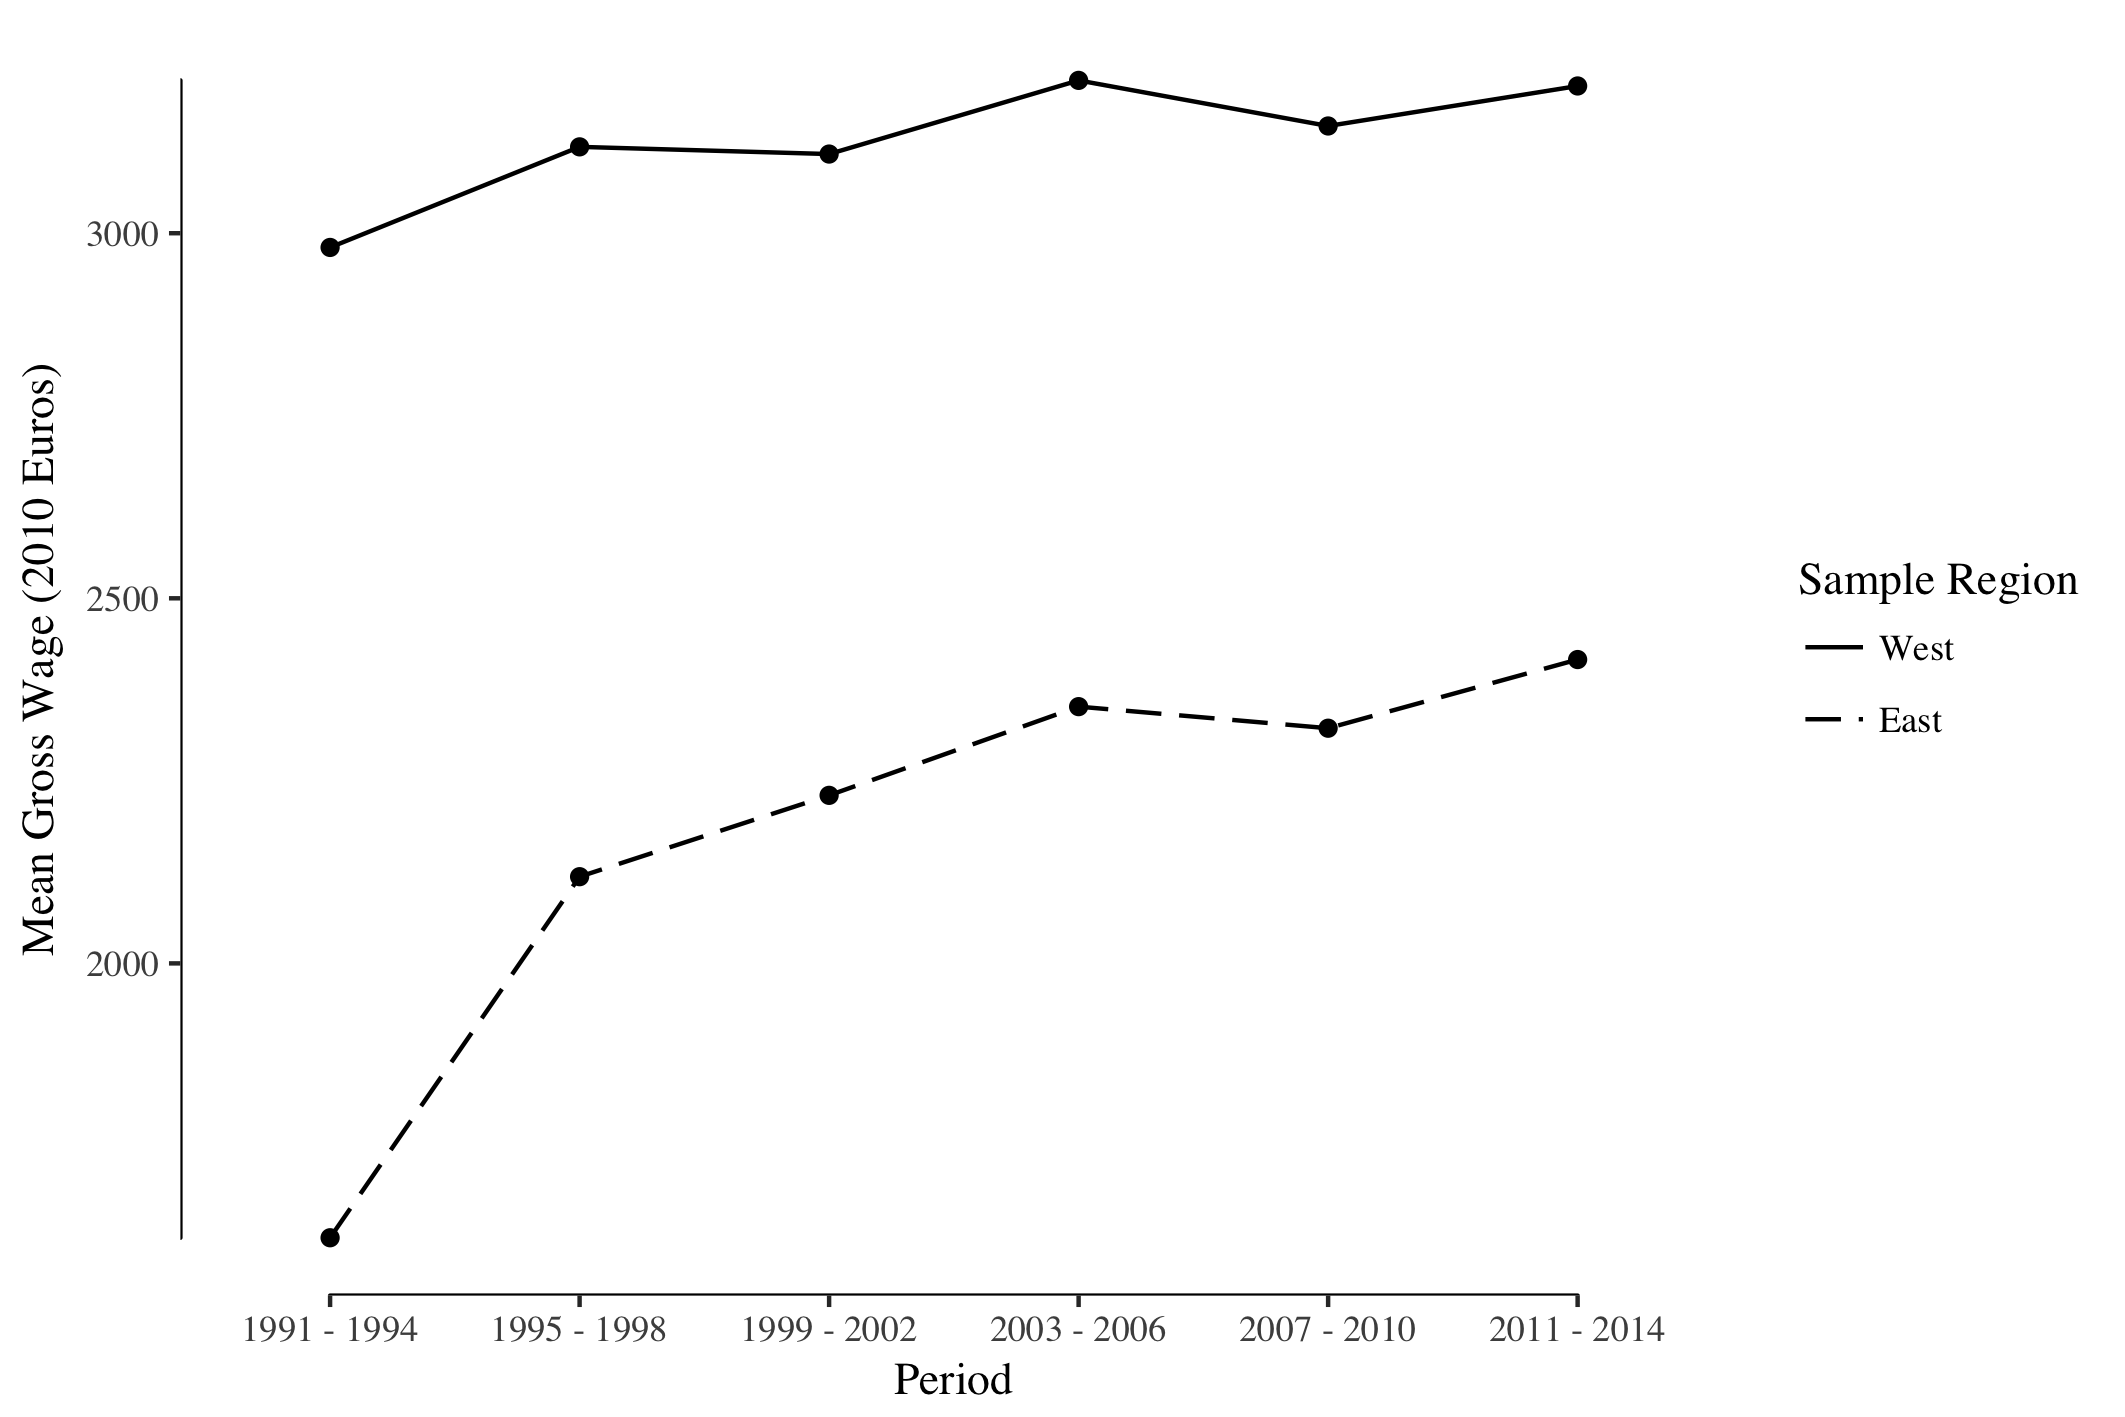
\includegraphics[width=0.8\textwidth]{/Users/Christian/Statistik_Studium/EconProject/Code/Graphics/plotMeanWages.png}
    \label{fig:MeanWages}
	\end{figure}
	\end{center}
}

\frame{
	\frametitle{Wage distribution across Total Experience significantly flatter in East Germany:}
	\begin{center}
	\begin{figure}[!h]
    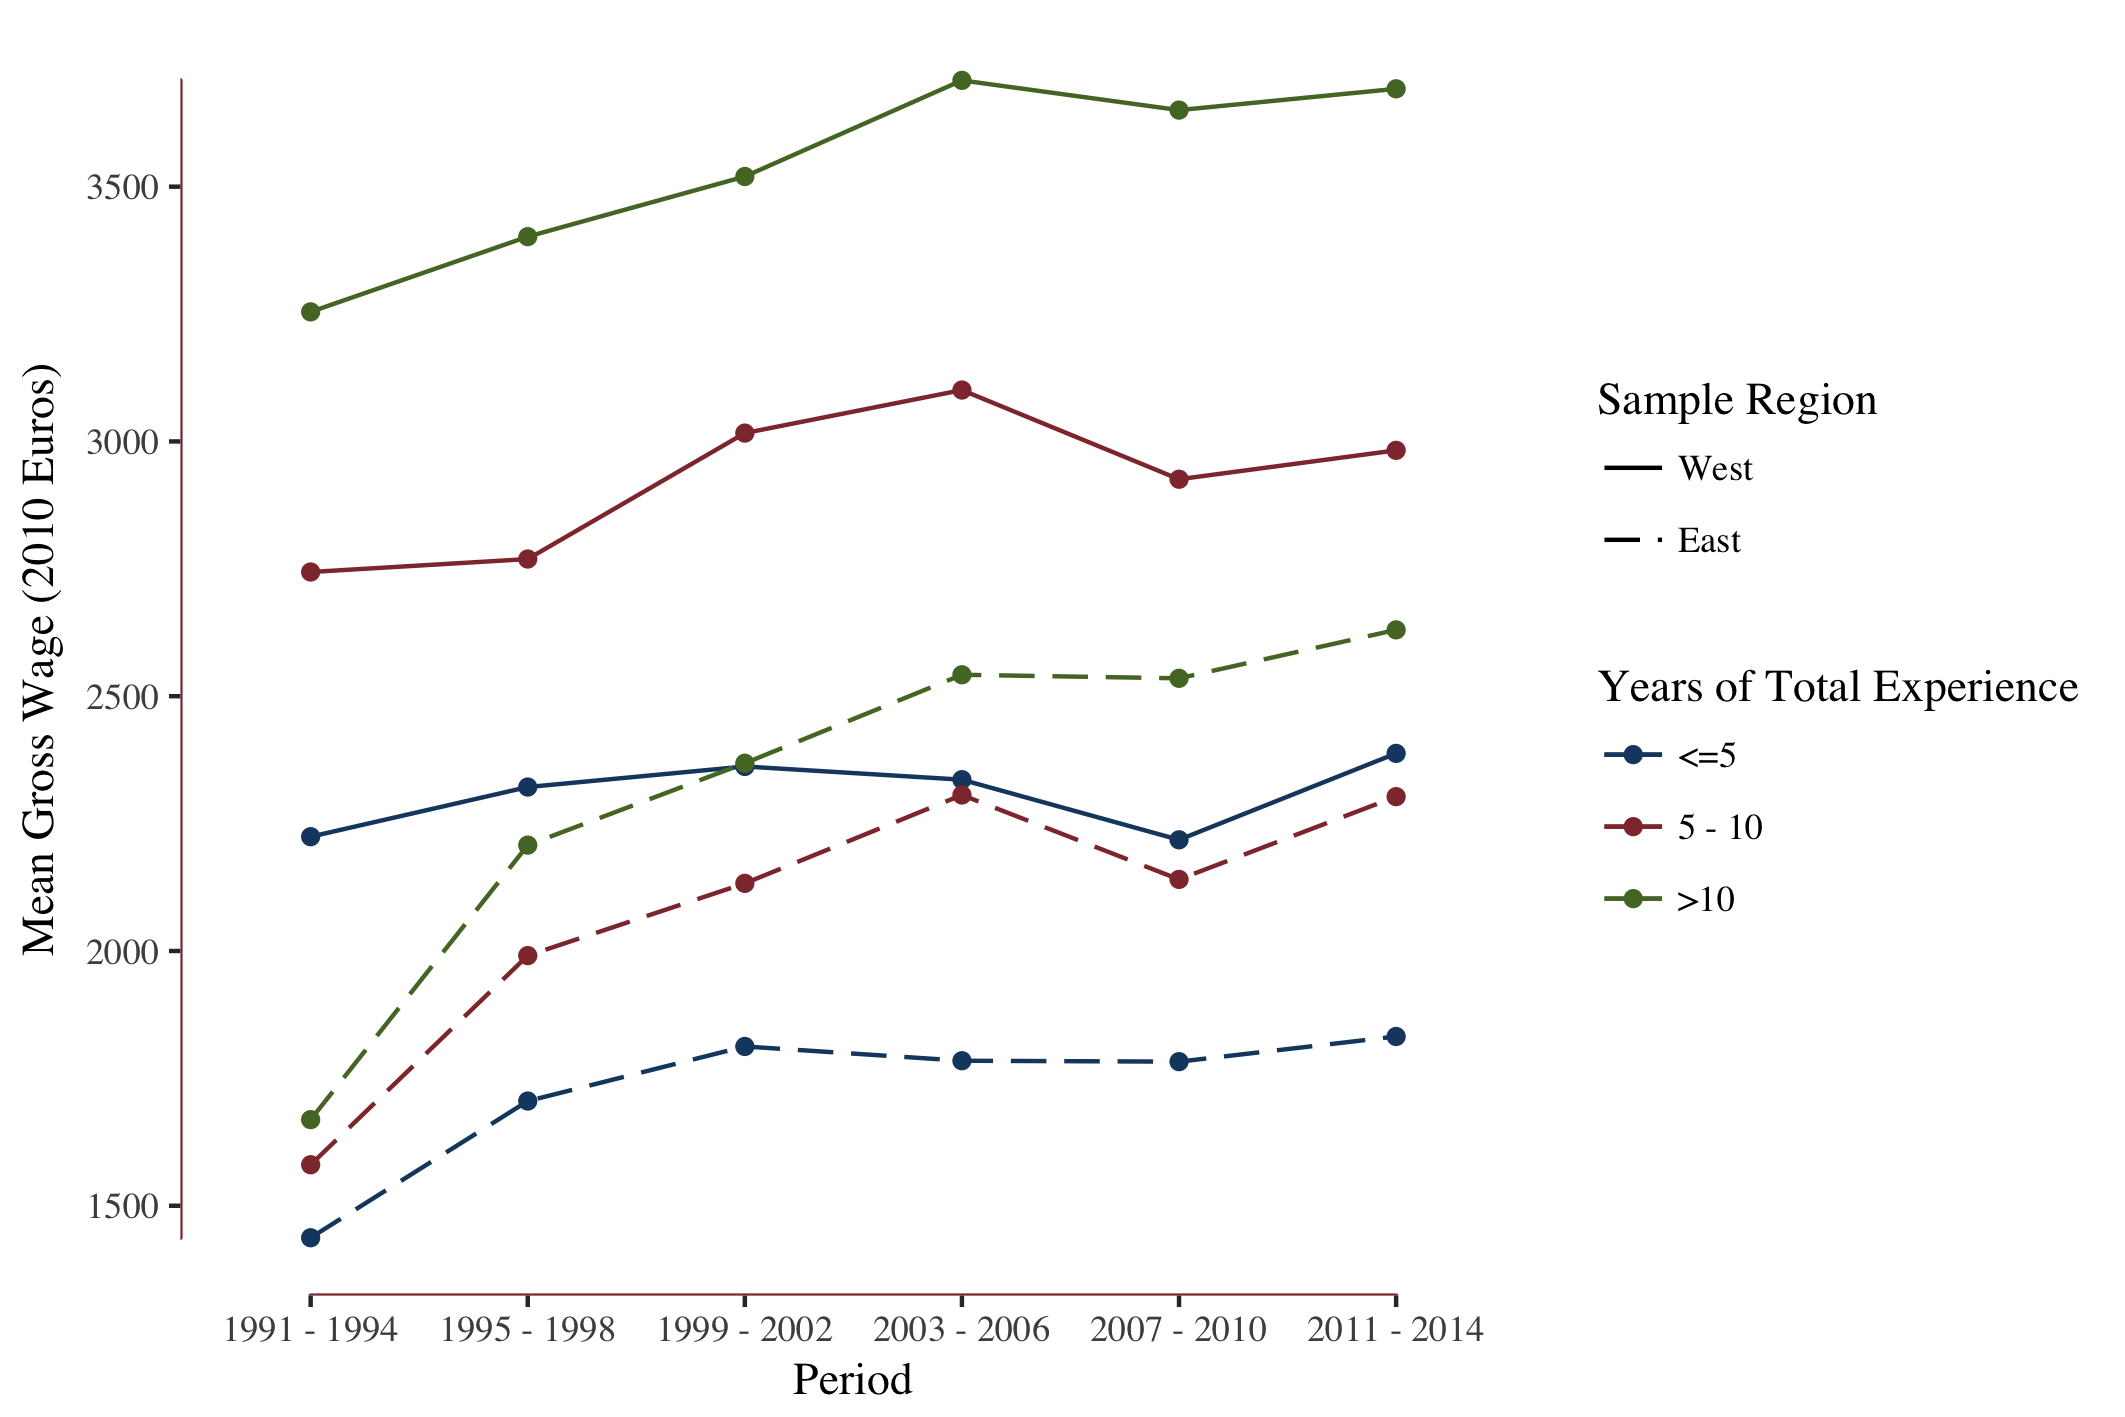
\includegraphics[width=0.8\textwidth]{/Users/Christian/Statistik_Studium/EconProject/Code/Graphics/plotMeanWagesByTotalExp.png}
    \label{fig:MeanWagesByTotalExp}
	\end{figure}
	\end{center}
}

\frame{
	\frametitle{Old Experience seems to have no effect on wages in East Germany:}
	\begin{center}
	\begin{figure}[!h]
    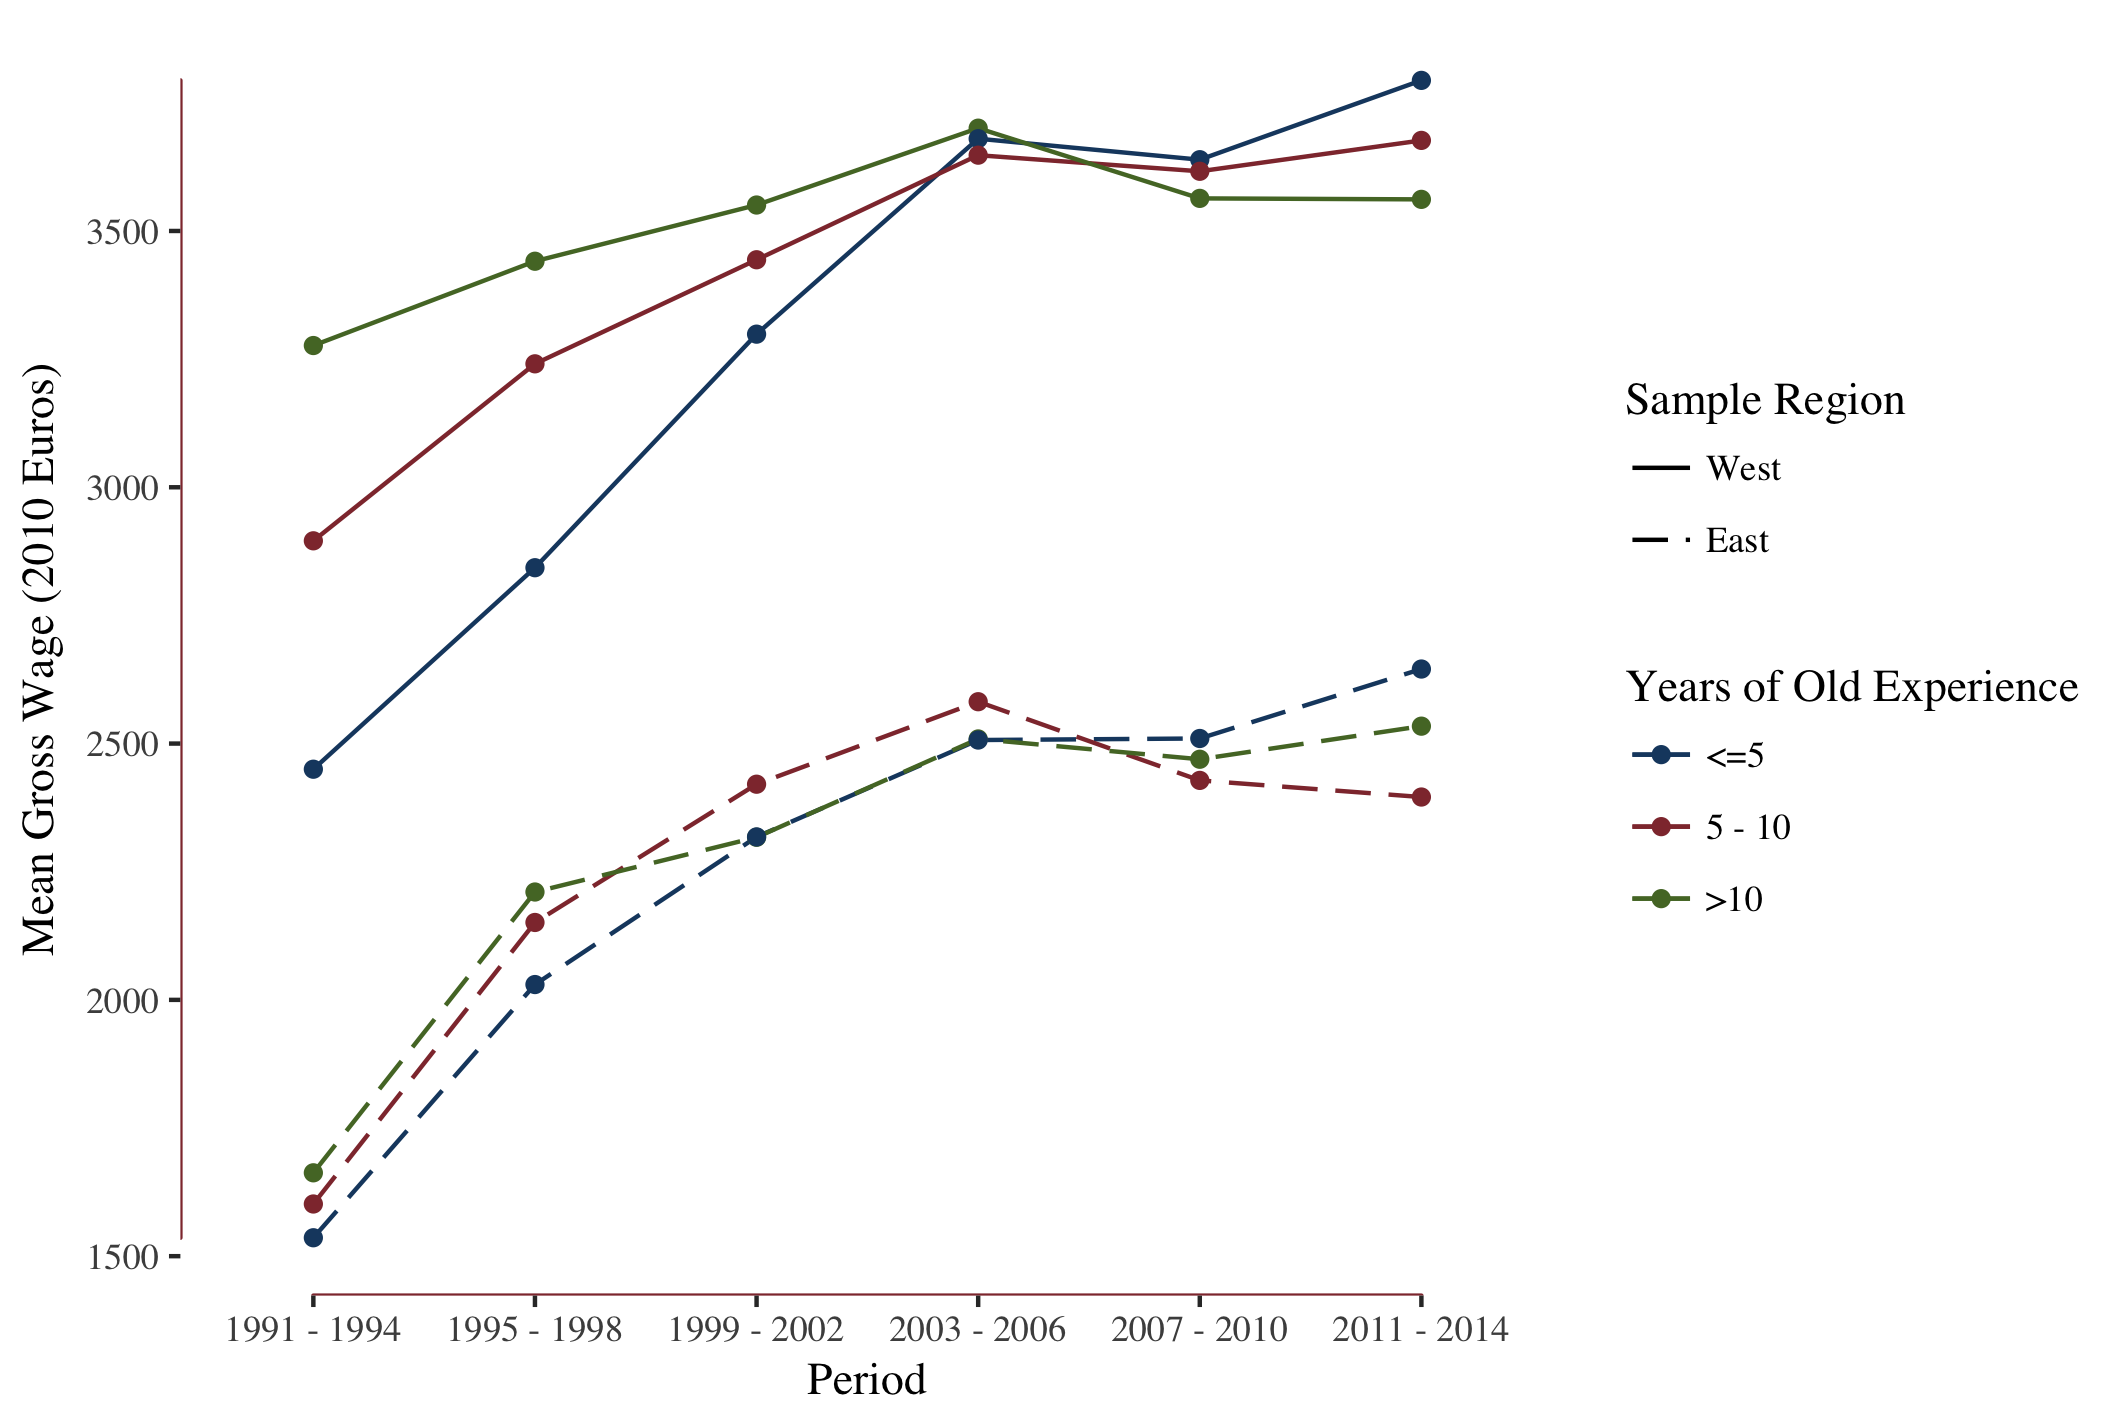
\includegraphics[width=0.8\textwidth]{/Users/Christian/Statistik_Studium/EconProject/Code/Graphics/plotMeanWagesByOldExp.png}
    \label{fig:MeanWagesByOldExp}
	\end{figure}
	\end{center}
}

\frame{
	\frametitle{Differences are much smaller regarding wage distribution across education:}
	\begin{center}
	\begin{figure}[!h]
    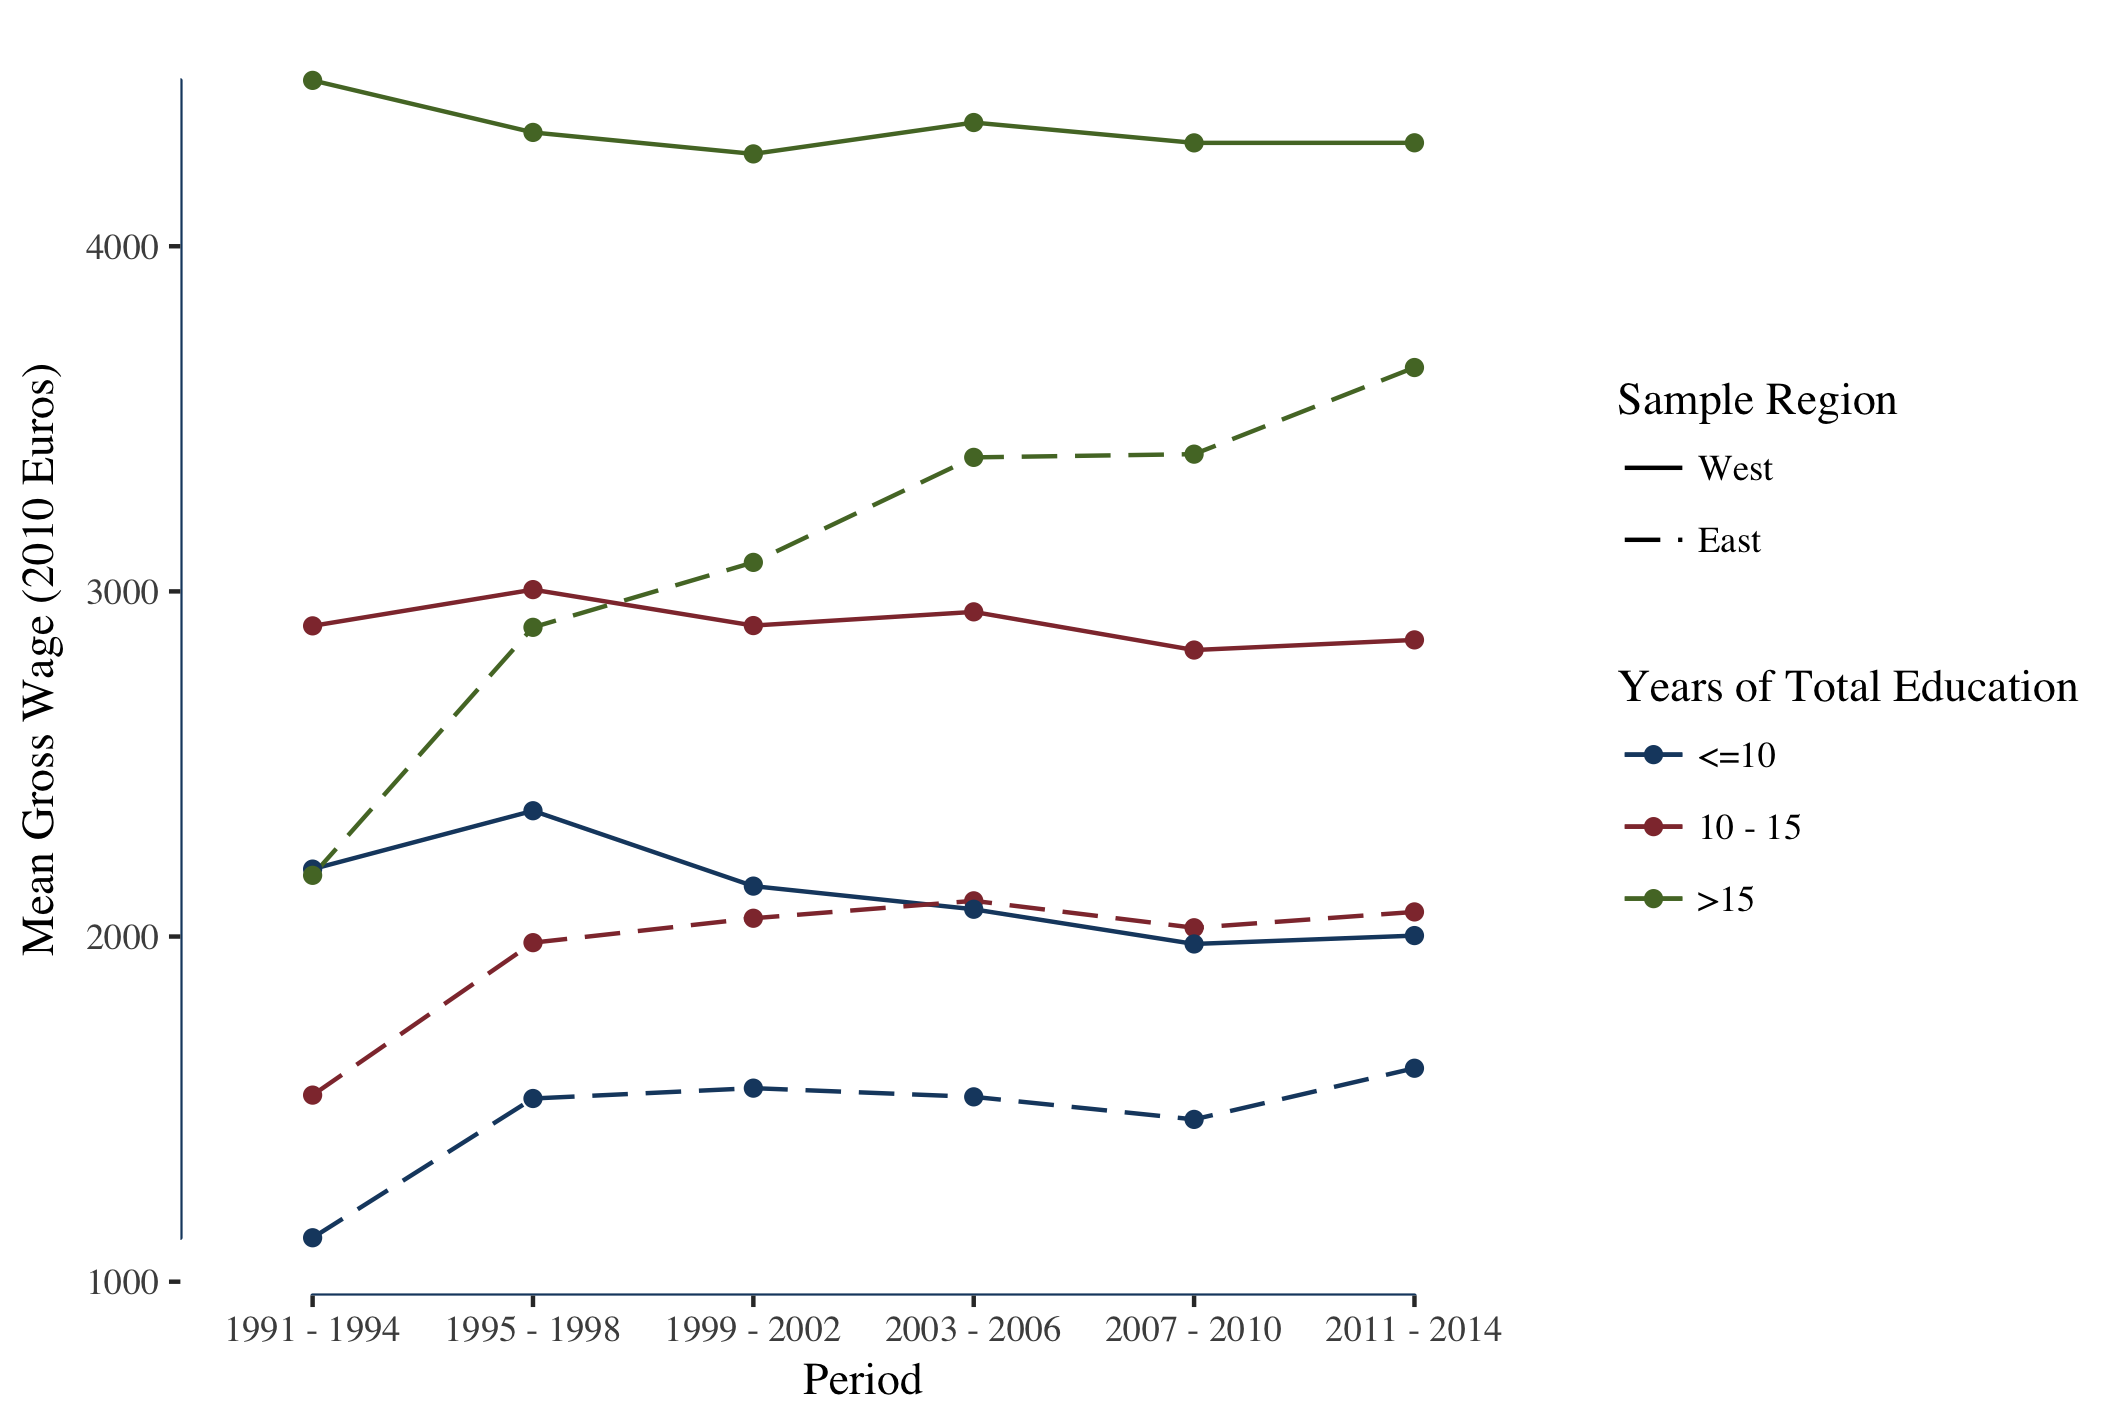
\includegraphics[width=0.8\textwidth]{/Users/Christian/Statistik_Studium/EconProject/Code/Graphics/plotMeanWagesByTotalEdu.png}
    \label{fig:MeanWagesByTotalEdu}
	\end{figure}
	\end{center}
}

\subsec{Explanatory Variables}
\frame{
	\tableofcontents[ 
	currentsubsection, 
	hideothersubsections, 
	sectionstyle= show/shaded,
	subsectionstyle= show/shaded, 
	] 
}
\frame{
	\frametitle{There is more Experience (especially Old one) in the East German sample:}
	\begin{center}
	\begin{figure}[!h]
    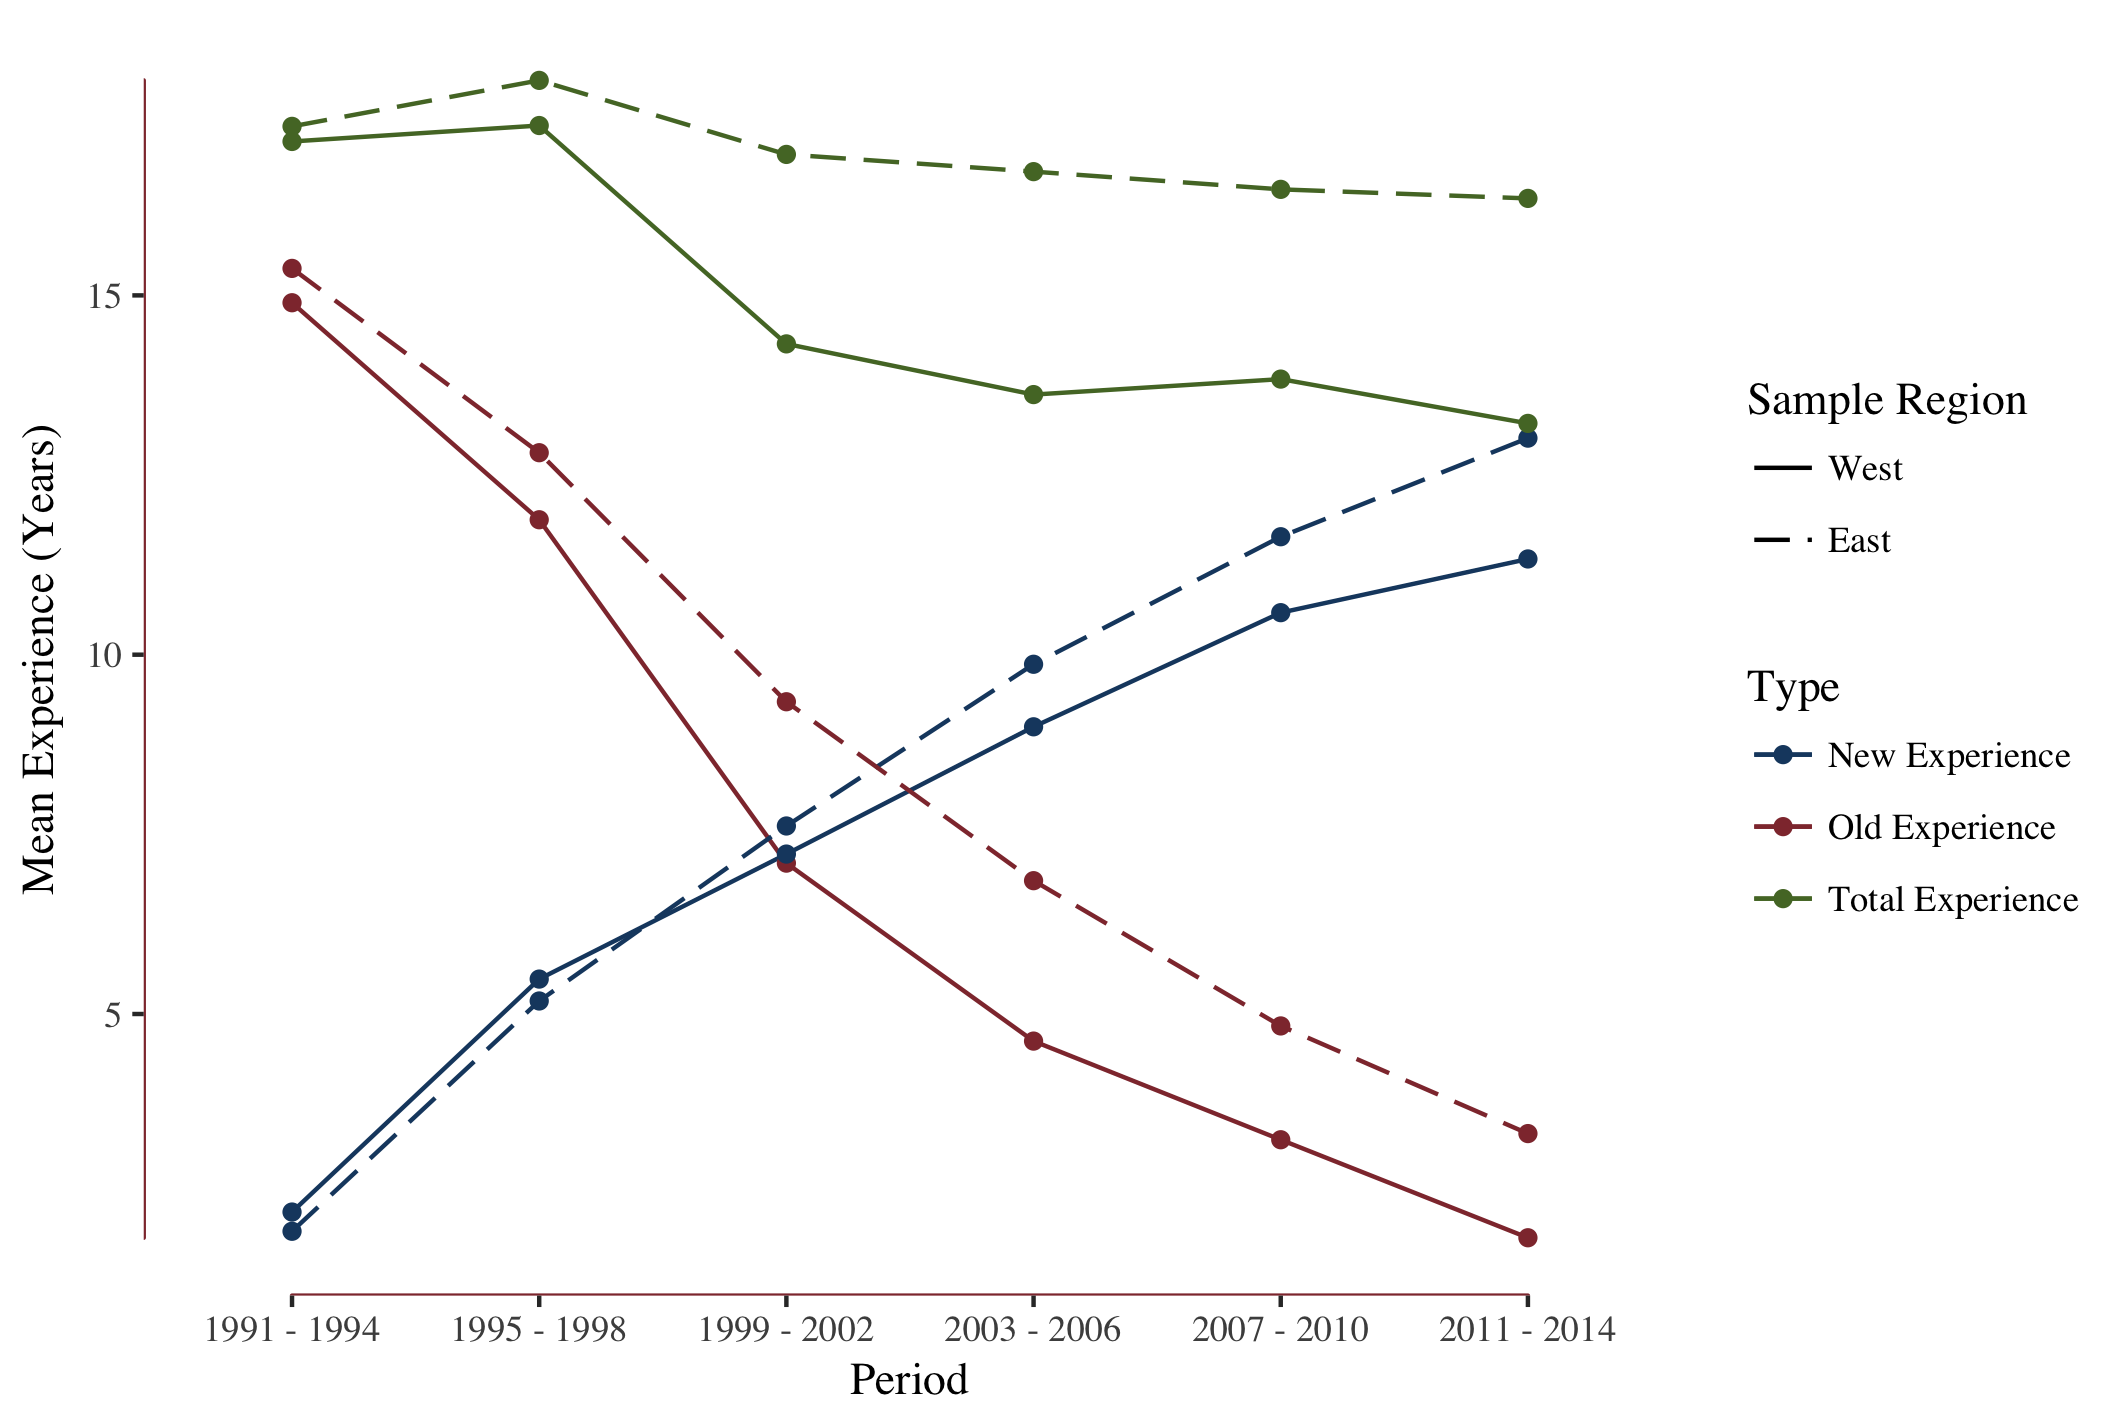
\includegraphics[width=0.8\textwidth]{/Users/Christian/Statistik_Studium/EconProject/Code/Graphics/plotMeanExp.png}
    \label{fig:MeanExp}
	\end{figure}
	\end{center}
}

\frame{
	\frametitle{Total Education levels are similar, but the share of Old Education is higher in the East:}
	\begin{center}
	\begin{figure}[!h]
    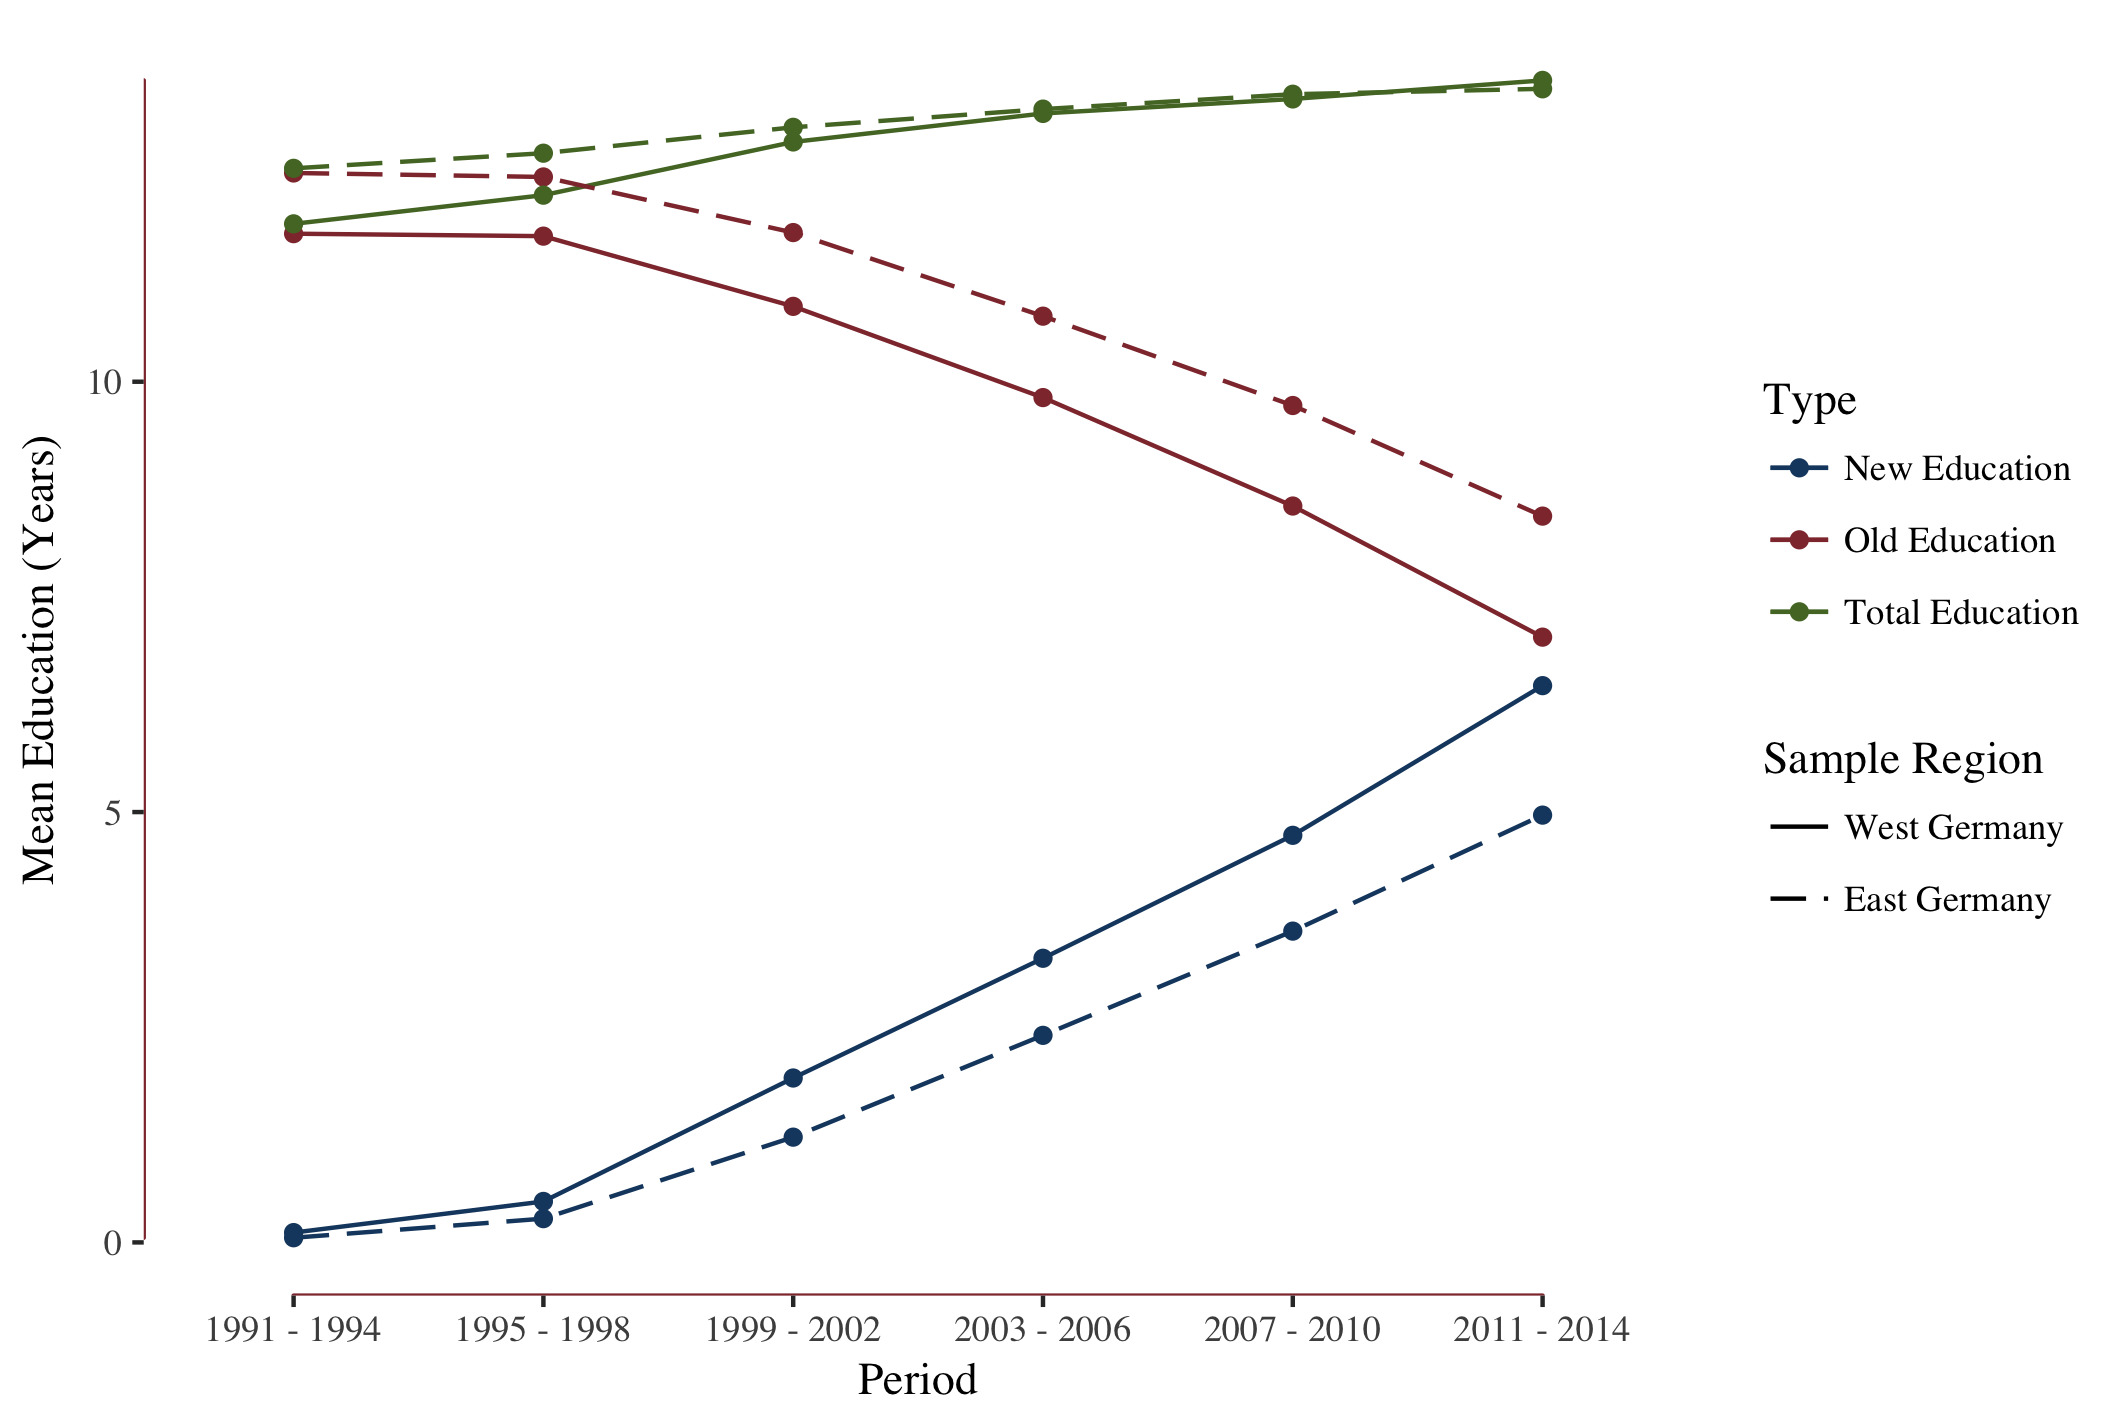
\includegraphics[width=0.8\textwidth]{/Users/Christian/Statistik_Studium/EconProject/Code/Graphics/plotMeanEdu.png}
    \label{fig:MeanEdu}
	\end{figure}
	\end{center}
}

\Section{Modelling}
\subsec{Model Equation}
\frame{
	\tableofcontents[ 
	currentsubsection, 
	hideothersubsections, 
	sectionstyle= show/shaded,
	subsectionstyle= show/shaded, 
	] 
}
\frame{
\frametitle{Two models are fitted to each of the subsets:}
\begin{equation}
	\begin{split}
	log(Wage) &= \beta_{1}TotalEdu + \beta_{2}TotalExp + \beta_{3} TotalExp^2\\
	&+\beta_{4}Tenure + \beta_{5}YearDummie + \beta_{6}Sex
	\end{split}
\end{equation}
\begin{equation} 
	\begin{split}
	log(Wage) &= \beta_{1a}OldEdu + \beta_{1b}NewEdu + \beta_{2a}OldExp \\
	&+ \beta_{2b}NewExp + \beta_{3a}OldExp^2 + \beta_{3b}NewExp^2\\
	&+\beta_{4}Tenure + \beta_{5}YearDummie + \beta_{6}Sex
	\end{split}
\end{equation}
}
\subsec{Estimation}
\frame{
	\tableofcontents[ 
	currentsubsection, 
	hideothersubsections, 
	sectionstyle= show/shaded,
	subsectionstyle= show/shaded, 
	] 
}
\frame{
\frametitle{These models are applied to the data in the following way:}
\begin{itemize}
	\item By fitting model 1 to the West German dataset of the years 1991 to 1994 we get coefficient: $\hat{\beta}_{2}^{(9194, West)}$ for the linear part of returns to total experience.
	\item The log wage differential 0 - 5 years in this dataset is then calculated as: $$Diff_{0-5,TotalExp}^{(9194, West)} = \hat{\beta}_{2}^{(9194, West)}*5 + \hat{\beta}_{3}^{(9194, West)} * 5^2$$
\end{itemize}
}
\frame{
\frametitle{These models are applied to the data in the following way:}
\begin{itemize}
	\item The mean log wage differential for total experience equals:
	\begin{equation} 
	\begin{split}
	Diff_{TotalExp}^{(9194, west)} =& \frac{1}{|I_{9194}^{west}|}\sum_{i \in 	I_{91-94}^{west}} \hat{\beta}_{2}^{(9194, west)}*TotalExp_{i}\\
 	&+\hat{\beta}_{3}^{(9194, west)} * TotalExp_{i}^2
	\end{split}
	\end{equation}
	\item Where $I_{9194}^{West}$ is the set of all observations in the respective subset.
\end{itemize}
}
\Section{Results}
\subsec{Global Analysis}
\frame{
	\tableofcontents[ 
	currentsubsection, 
	hideothersubsections, 
	sectionstyle= show/shaded,
	subsectionstyle= show/shaded, 
	] 
}
\frame{
\frametitle{Returns to Education:}
\begin{center}
\begin{figure}[!h]
    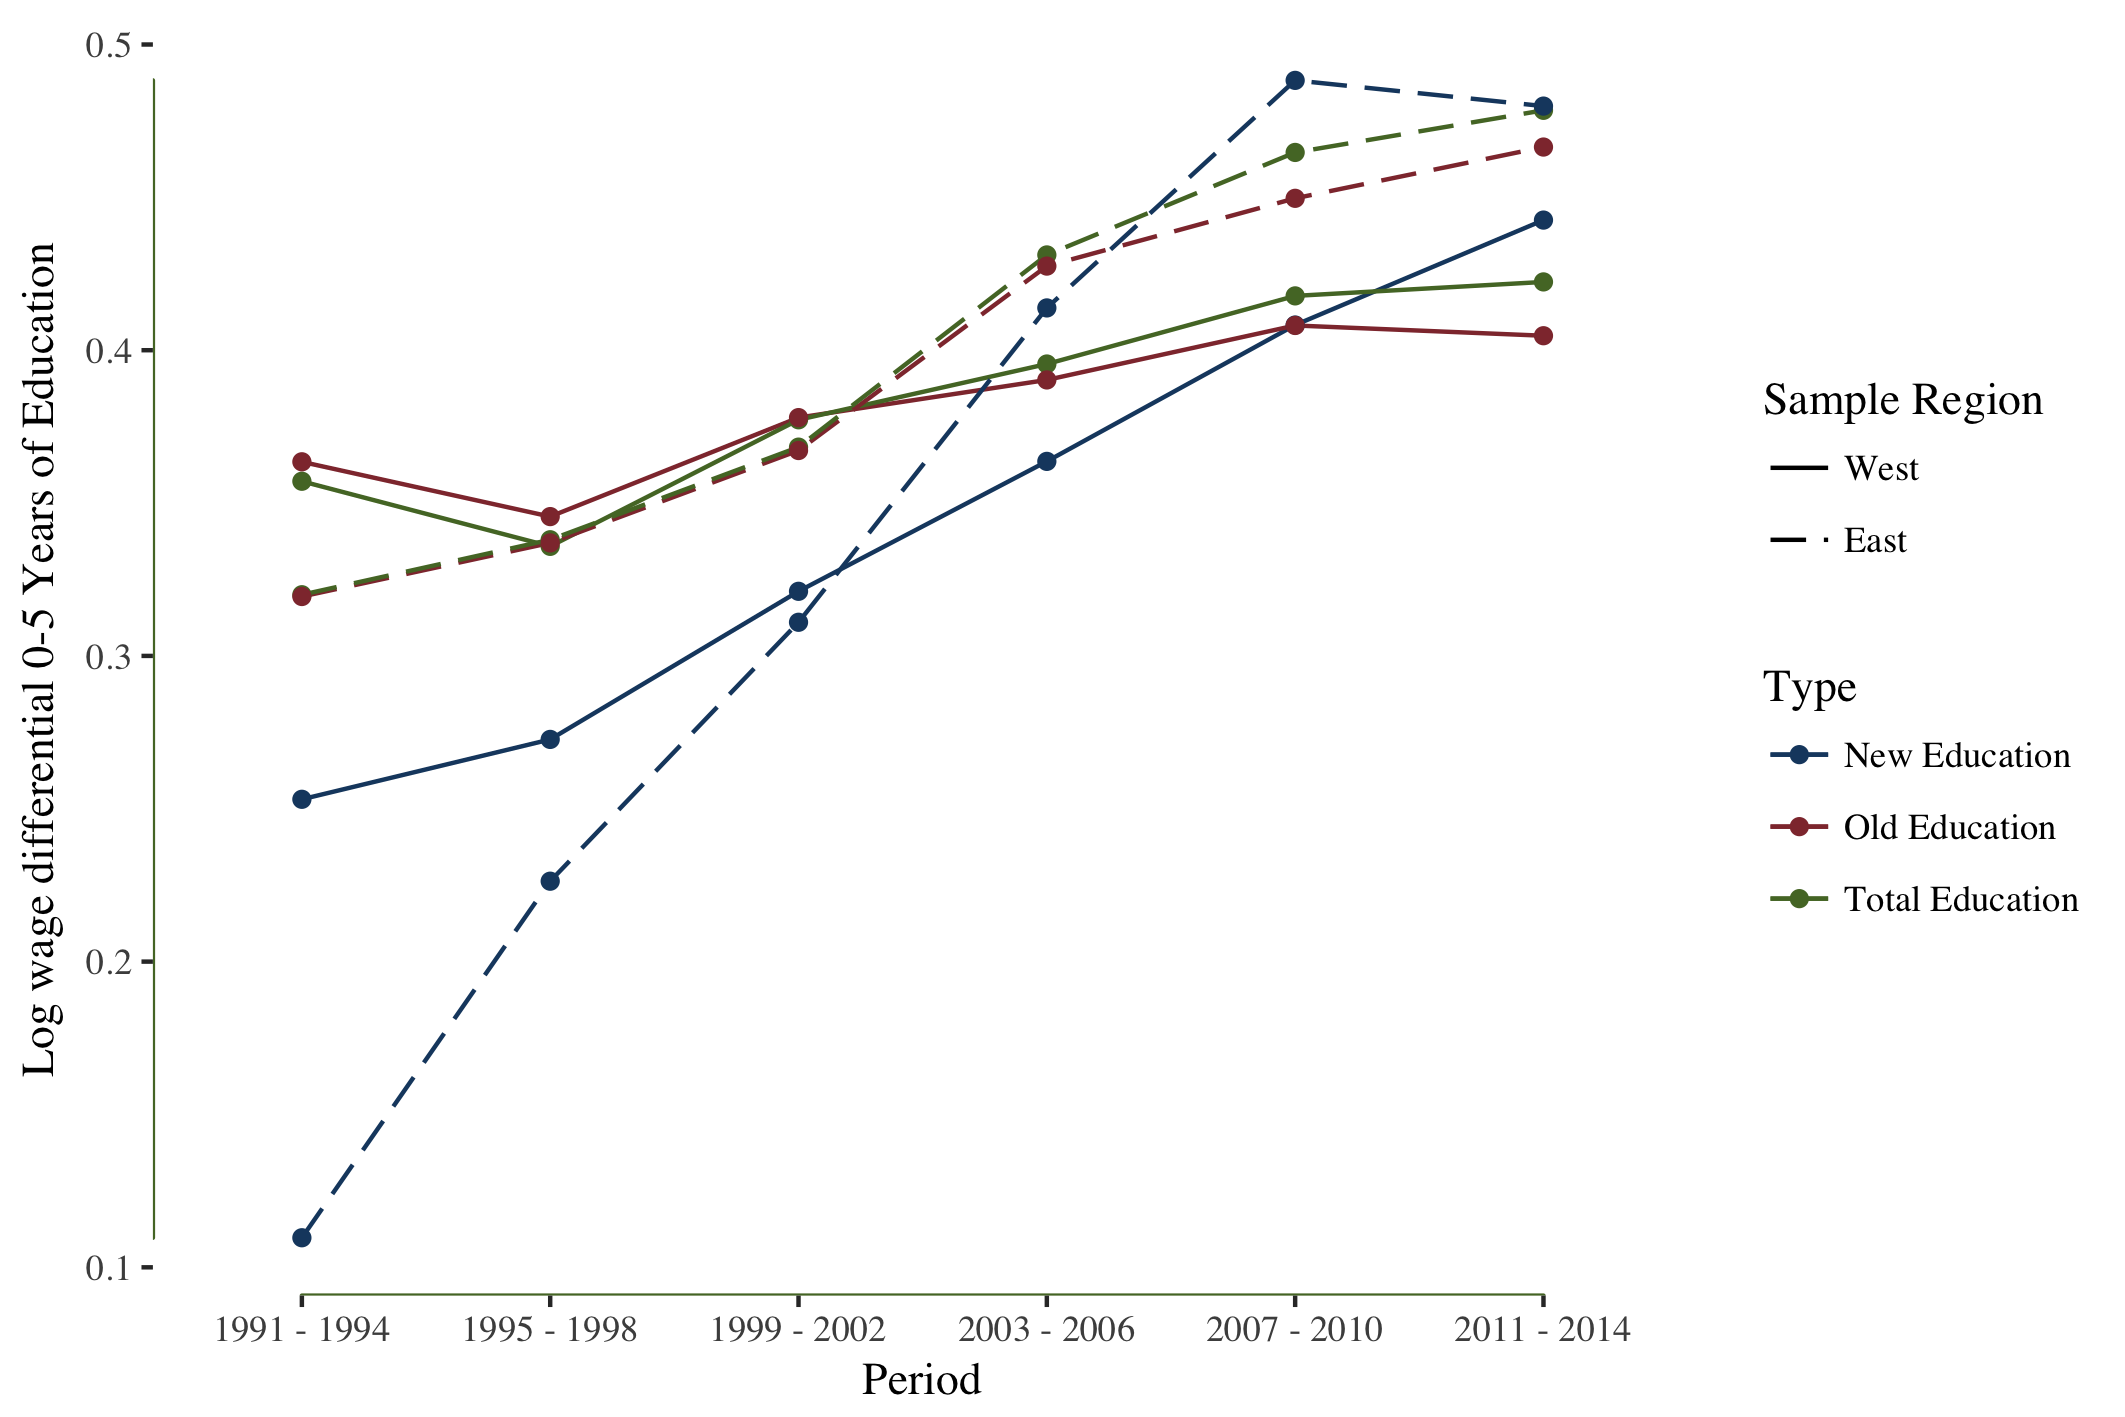
\includegraphics[width=0.8\textwidth]{/Users/Christian/Statistik_Studium/EconProject/Code/Graphics/plotDiffComparisonEdu.png}
    \label{fig:DiffComparisonEdu}
\end{figure}
\end{center}
}
\frame{
\frametitle{Returns to Experience:}
\begin{center}
\begin{figure}[!h]
    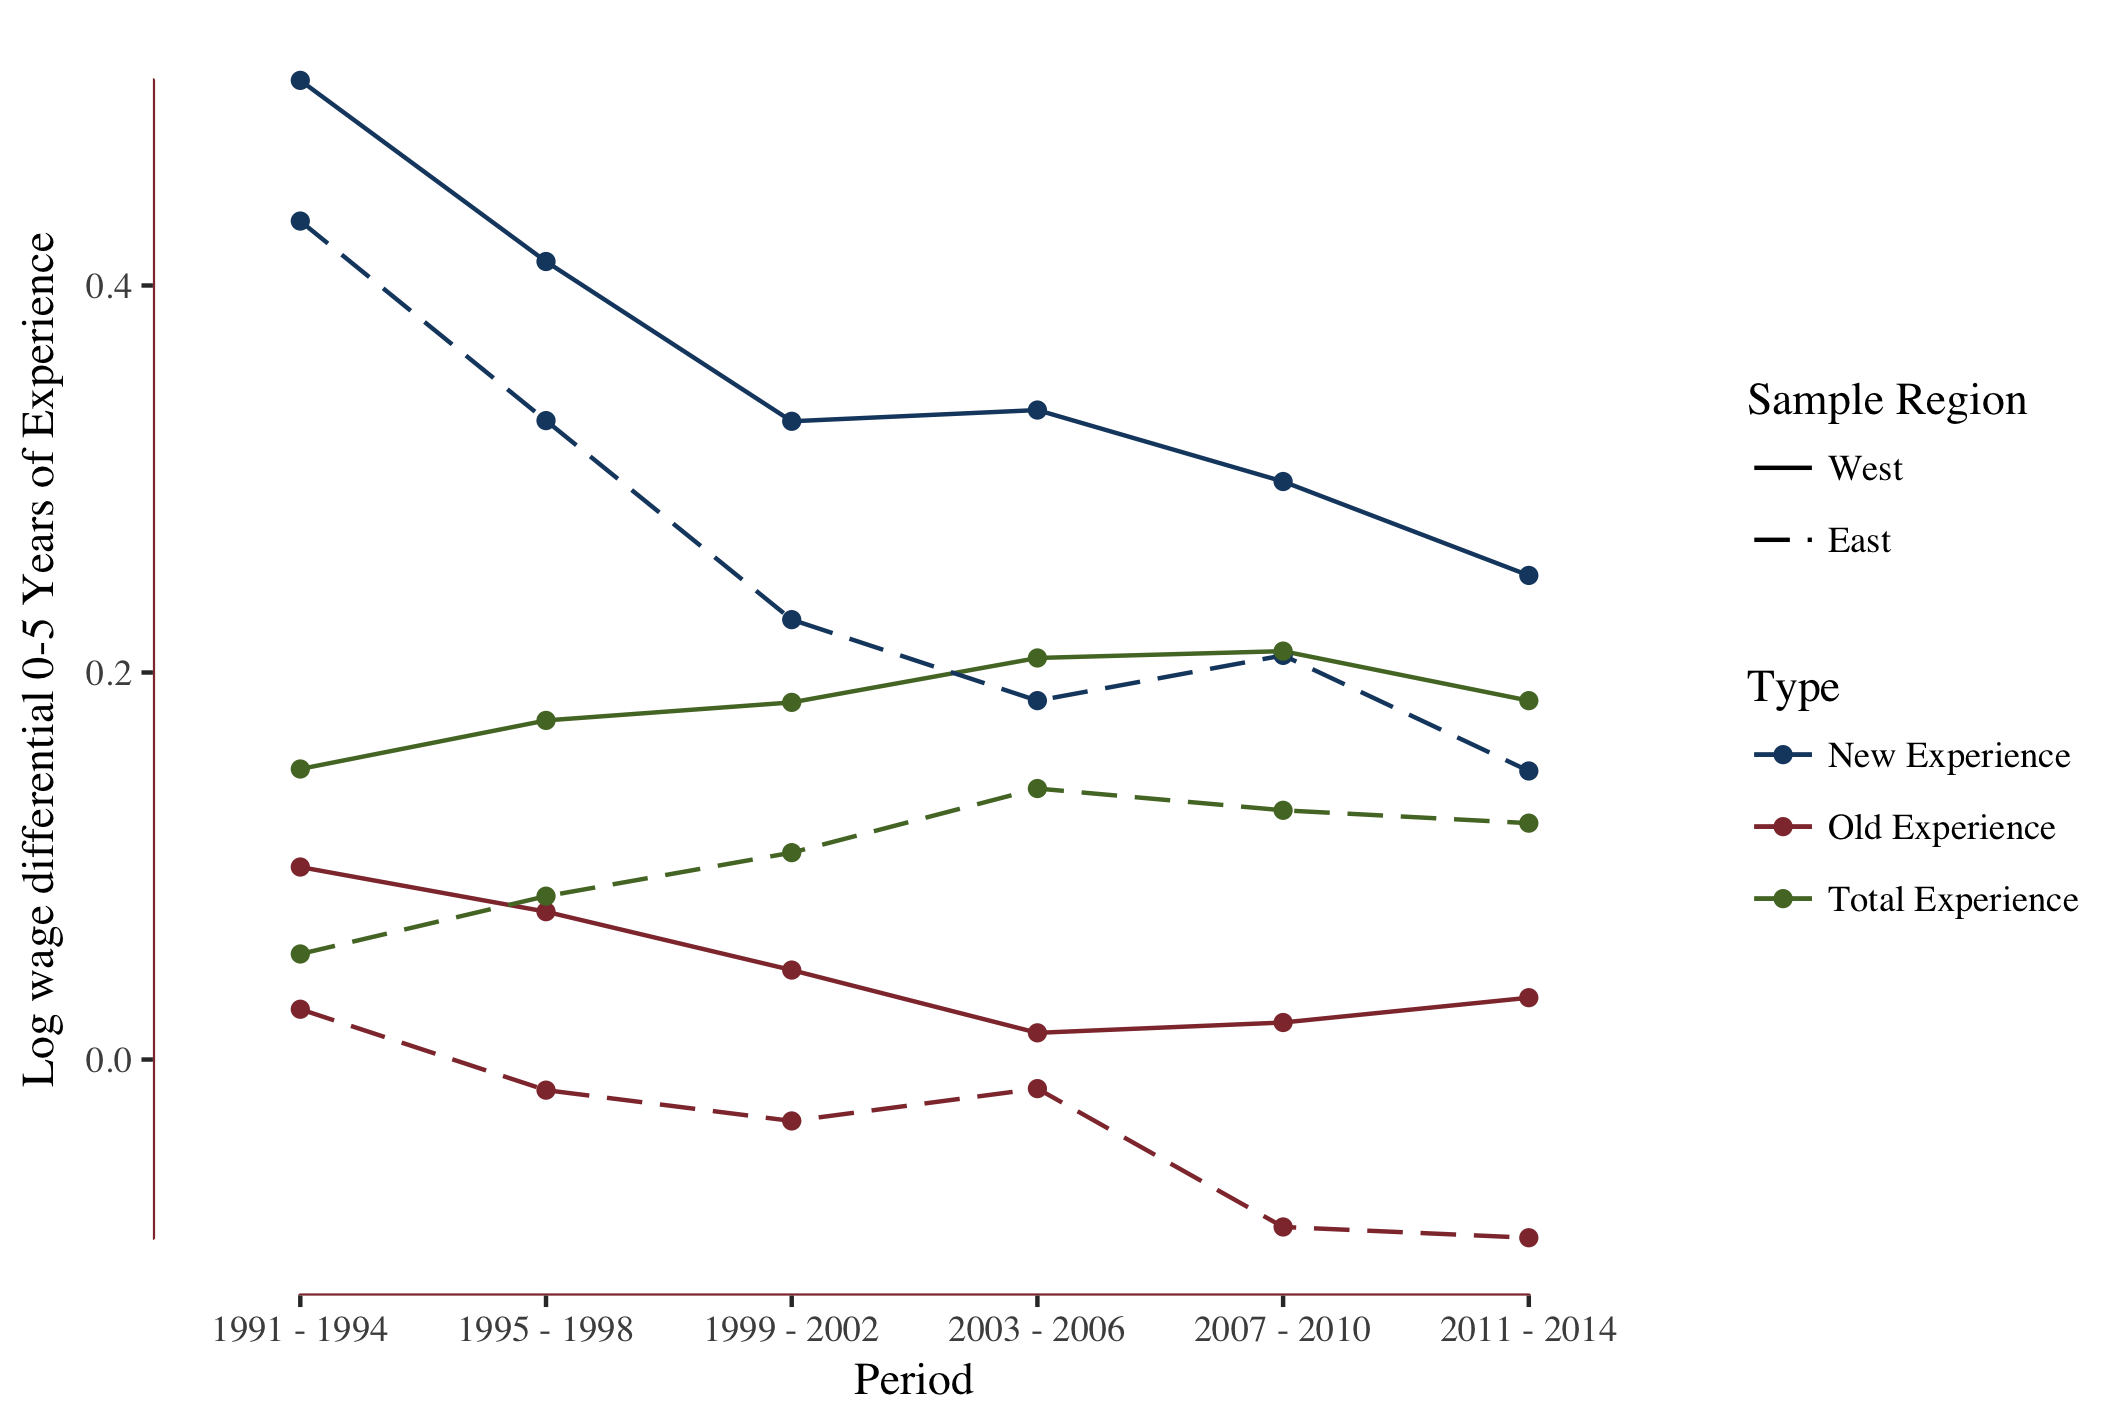
\includegraphics[width=0.8\textwidth]{/Users/Christian/Statistik_Studium/EconProject/Code/Graphics/plotDiffComparisonExp.png}
    \label{fig:DiffComparisonExp}
\end{figure}
\end{center}
}
\frame{
\frametitle{Human Capital in Education:}
\begin{center}
\begin{figure}[!h]
    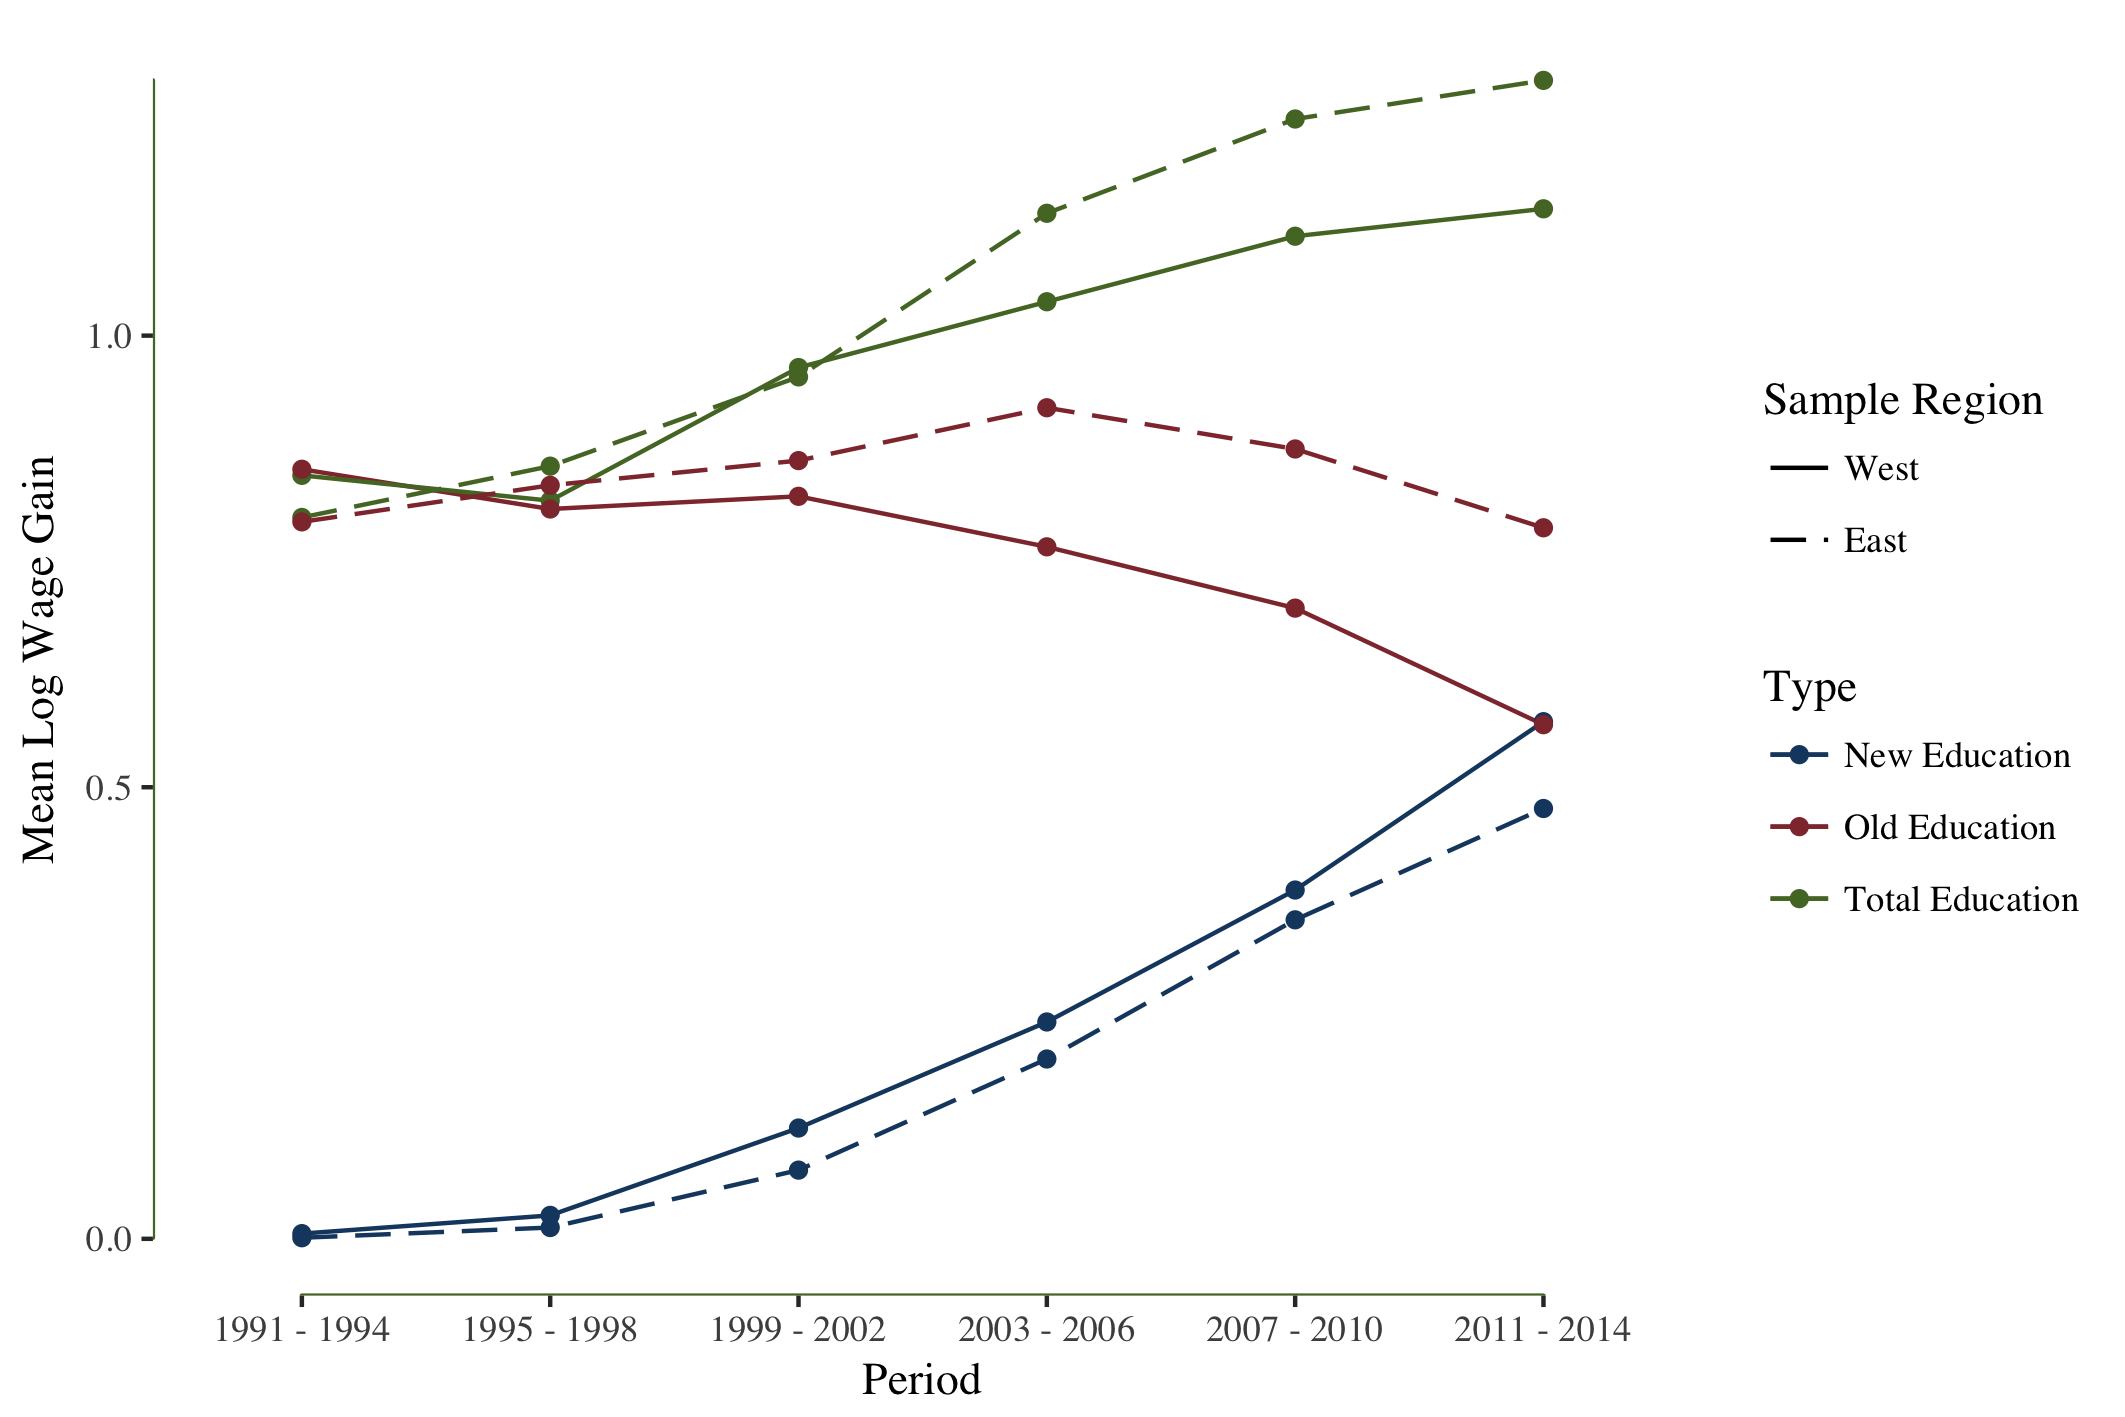
\includegraphics[width=0.8\textwidth]{/Users/Christian/Statistik_Studium/EconProject/Code/Graphics/plotHumanCapitalEdu.png}
    \label{fig:HumanCapitalEdu}
\end{figure}
\end{center}
}

\frame{
\frametitle{Human Capital in Experience:}
\begin{center}
\begin{figure}[!h]
    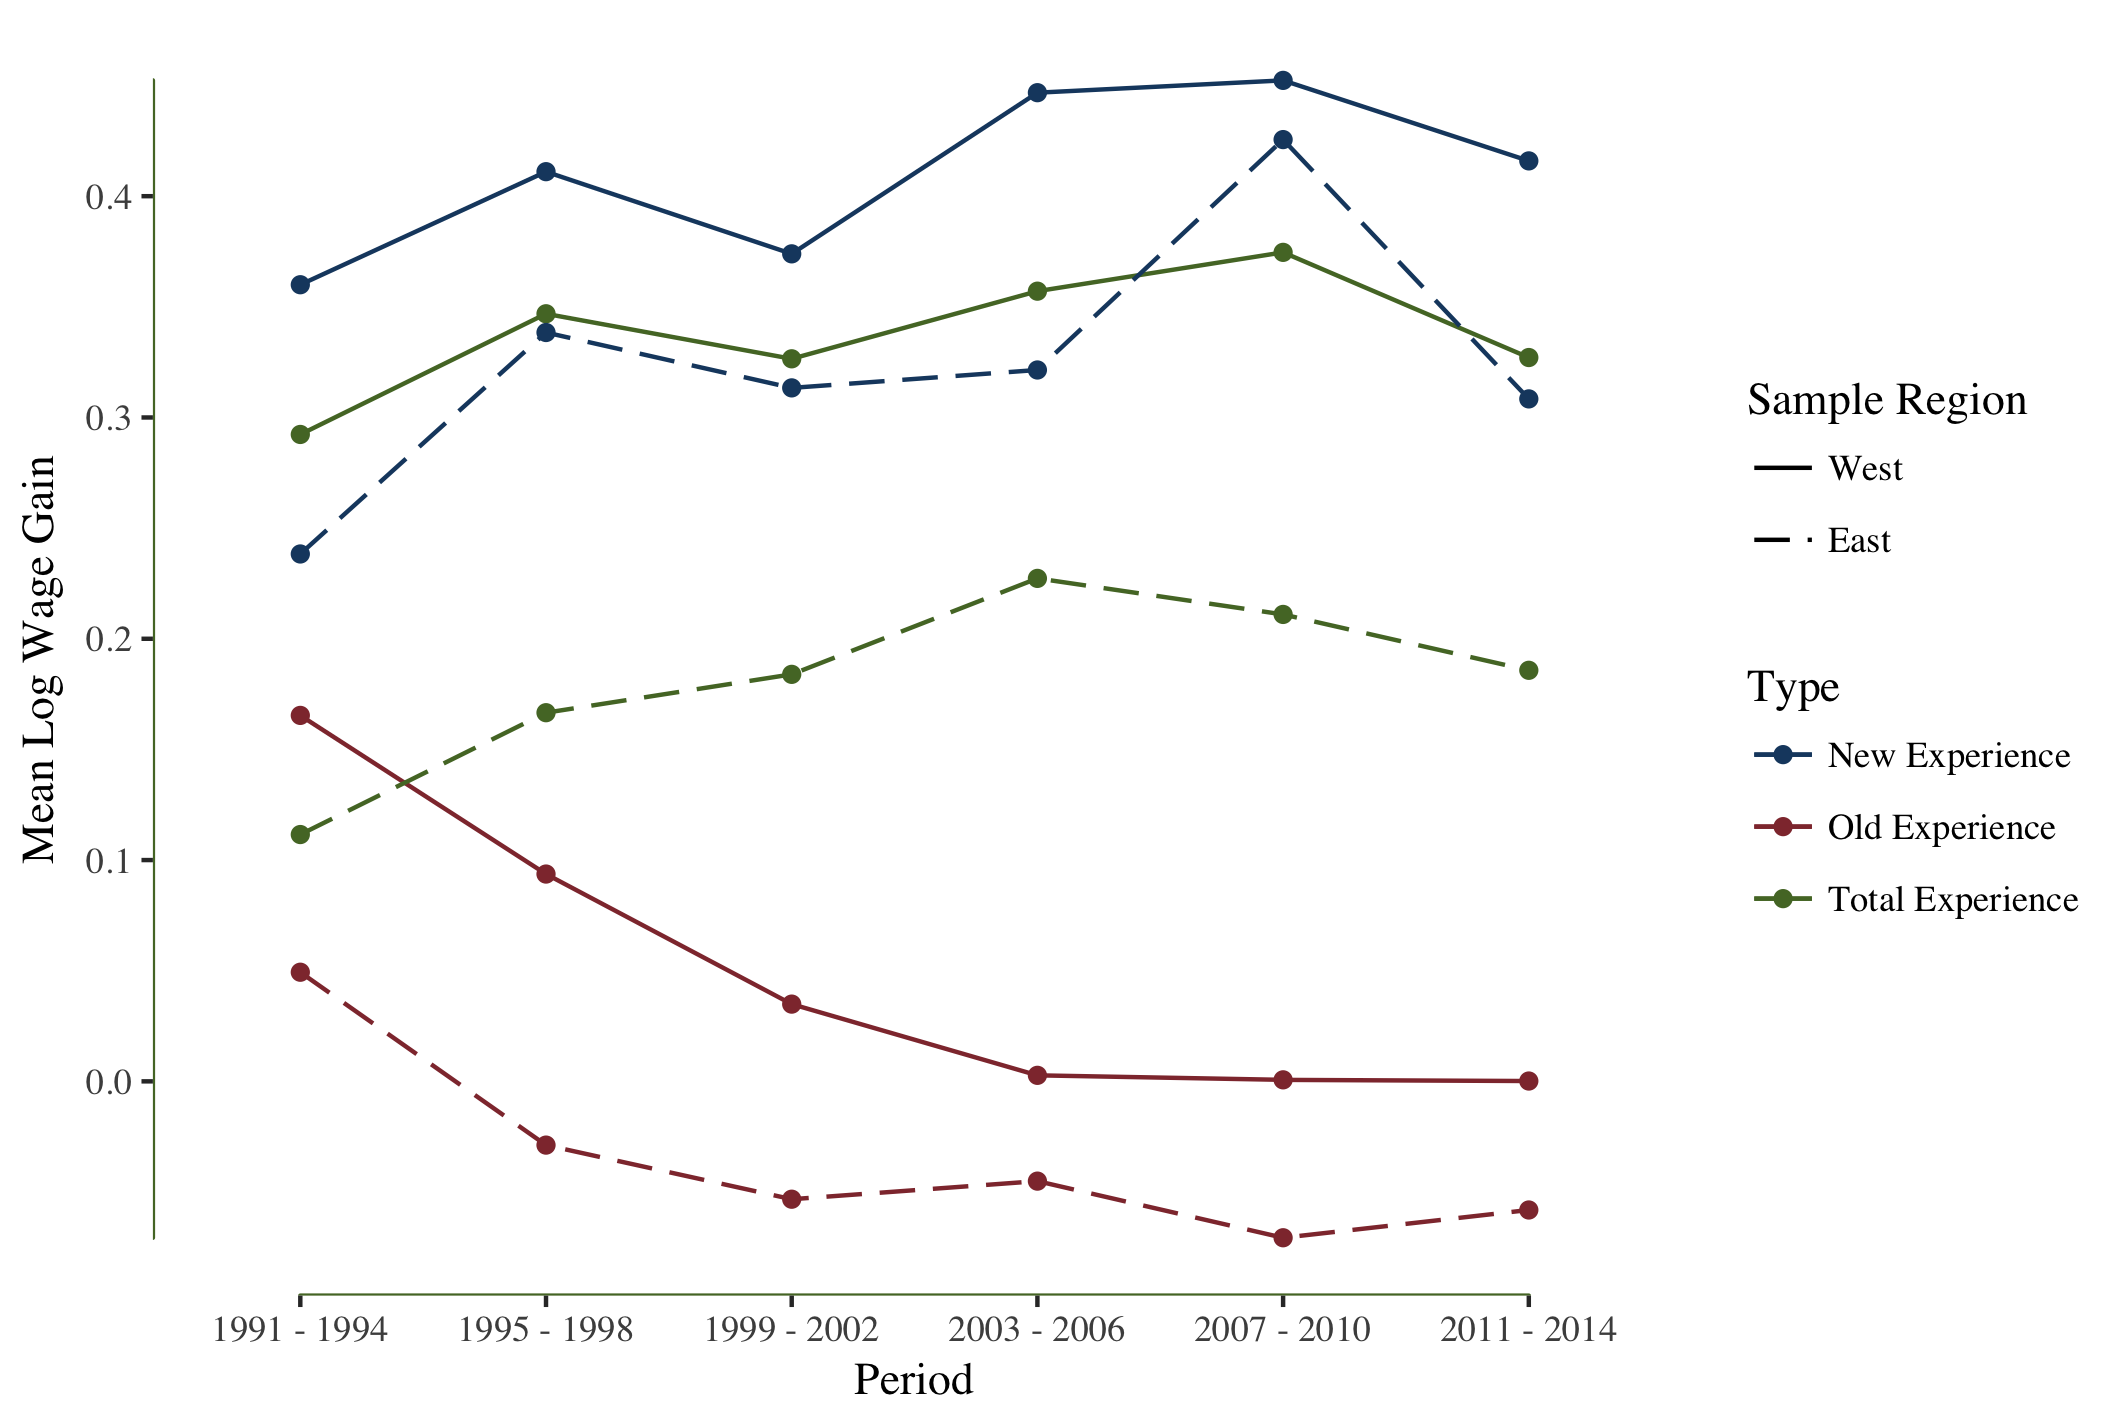
\includegraphics[width=0.8\textwidth]{/Users/Christian/Statistik_Studium/EconProject/Code/Graphics/plotHumanCapitalExp.png}
    \label{fig:HumanCapitalExp}
\end{figure}
\end{center}
}


\subsec{Analysis by Skill Group}
\frame{
	\tableofcontents[ 
	currentsubsection, 
	hideothersubsections, 
	sectionstyle= show/shaded,
	subsectionstyle= show/shaded, 
	] 
}
\frame{
\frametitle{Returns to Experience By Skill Group:}
\begin{center}
\begin{figure}[!h]
    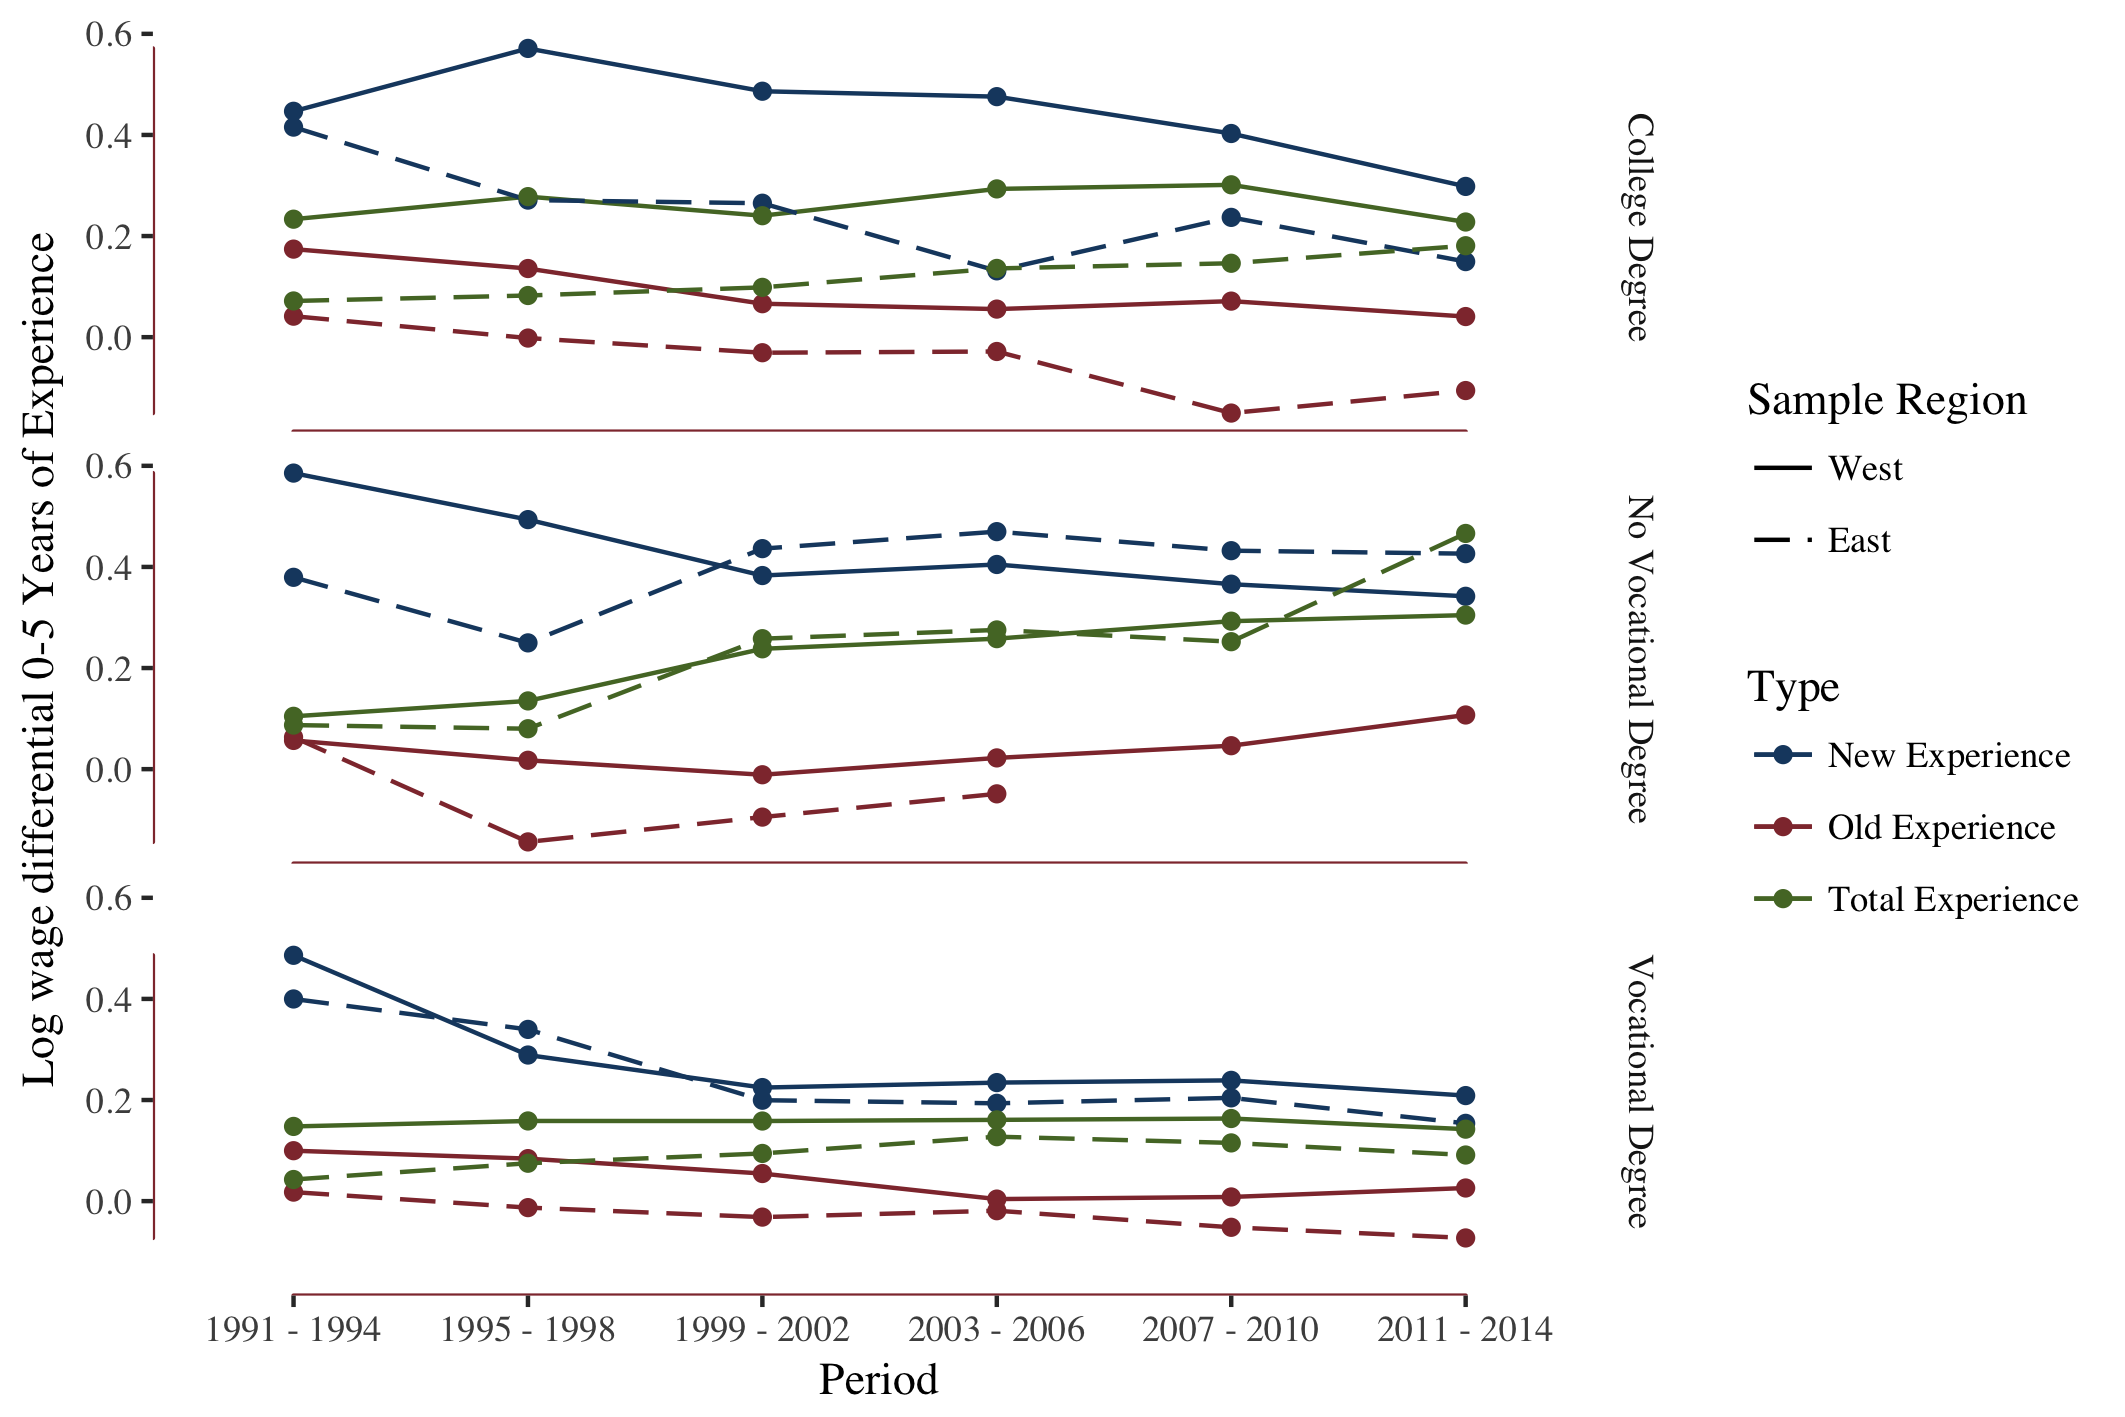
\includegraphics[width=0.8\textwidth]{/Users/Christian/Statistik_Studium/EconProject/Code/Graphics/plotDiffComparisonExpBySkillGroup.png}
    \label{fig:DiffComparisonExpBySkillGrou}
\end{figure}
\end{center}
}

\frame{
\frametitle{Human Capital in Experience By Skill Group:}
\begin{center}
\begin{figure}[!h]
    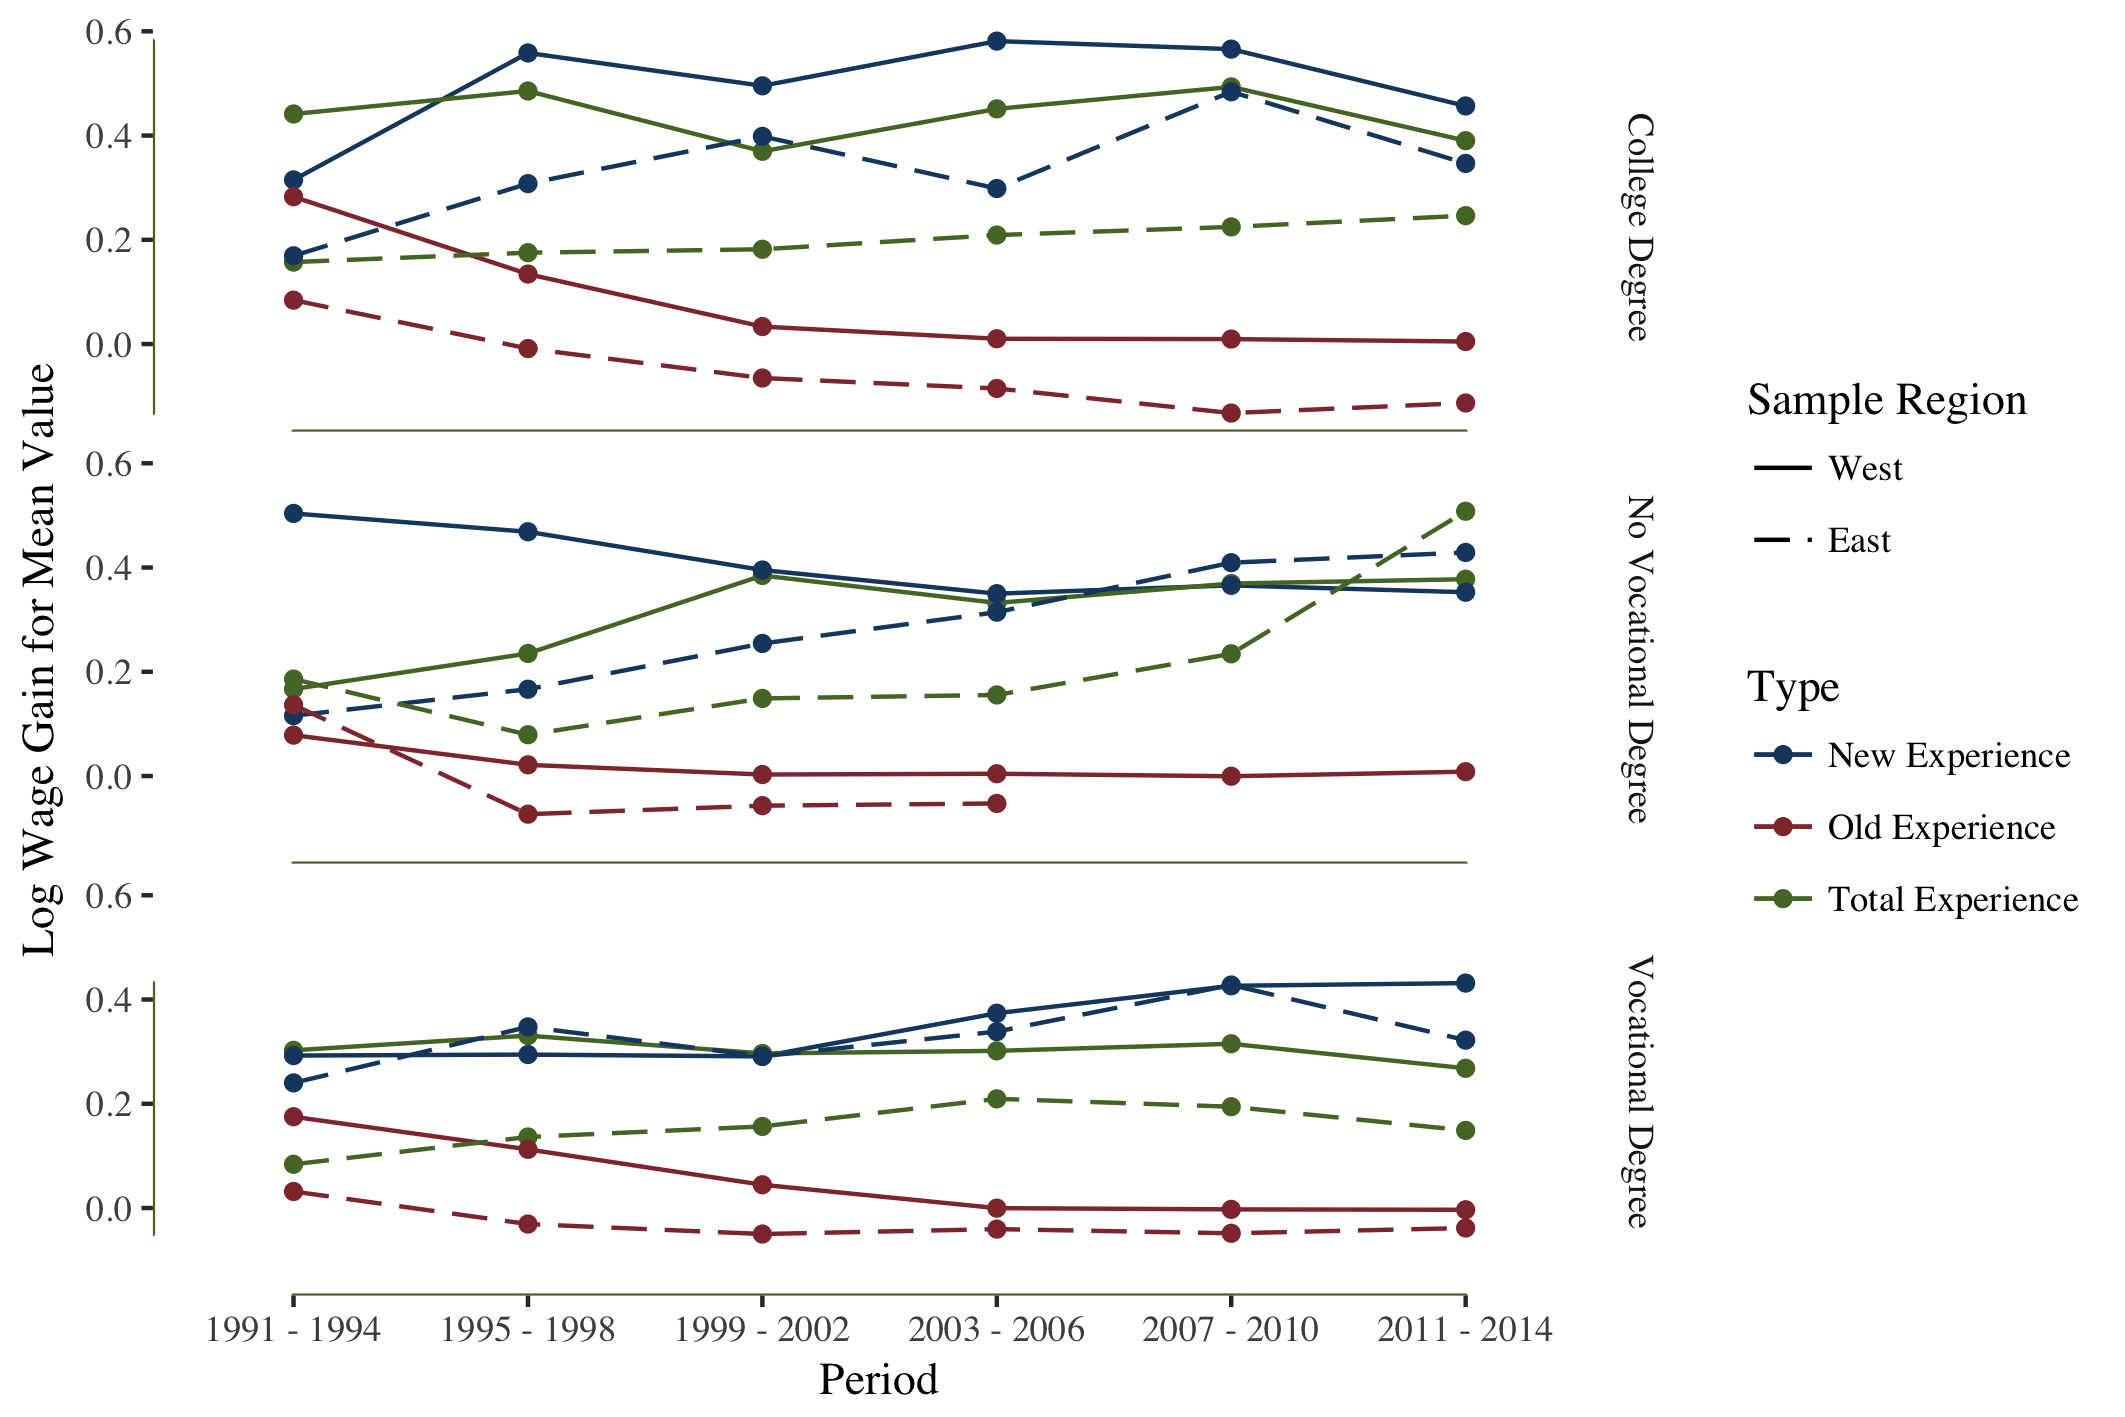
\includegraphics[width=0.8\textwidth]{/Users/Christian/Statistik_Studium/EconProject/Code/Graphics/plotHumanCapitalExpBySkillGroup.png}
    \label{fig:HumanCapitalExpBySkillGrou}
\end{figure}
\end{center}
}
\subsec{Conclusion}
\frame{
	\tableofcontents[ 
	currentsubsection, 
	hideothersubsections, 
	sectionstyle= show/shaded,
	subsectionstyle= show/shaded, 
	] 
}
\begin{frame}[allowframebreaks]
\frametitle{From the above evidence one might draw the following conclusions regarding the research questions:}
\begin{enumerate}
	\item How do returns to education and experience differ in East and West Germany ?
	\begin{itemize}
		\item Returns to education (Old and New) show now significant differences
		\item Old Experience in East Germany loses its value immediately after reunification, whereas the devaluation in the West happens more gradually.
		\item The relative returns to New Experience are significantly higher in the West.
	\end{itemize}
	\item How do these differences develop over time ?
		\begin{itemize}
		\item Differences in Evaluation of Old Experience disappear over time, whereas differences regarding New Experience persist
		\item The remaining difference in valuation of Total Experience seem to be caused in the difference of evaluation of new experience.
		\end{itemize}
	\item How do these differences behave when differentiating between Experience and Education obtained pre- / post-unification?
		\begin{itemize}
			\item See above.
		\end{itemize}
	\item How do results vary for different Skill Groups ? (No Degree, Vocational- , College Degree)
		\begin{itemize}
		\item Initially large differences in returns to experience decreased much faster for individuals without degree than for those with college degree. 
		\item Differences in the returns to experience for individuals with vocational degree are relatively small throughout the time frame.
		\item The difference in human capital from New Experience seems to be concentrated in the group of people with College Degree.
		\end{itemize}
\end{enumerate}
\end{frame}

\beamertemplatebookbibitems
\begin{frame}[allowframebreaks]
\frametitle{References}
\bibliographystyle{apalike}
\bibliography{EconometricProject}
\end{frame}

\end{document}

